% Options for packages loaded elsewhere
% Options for packages loaded elsewhere
\PassOptionsToPackage{unicode}{hyperref}
\PassOptionsToPackage{hyphens}{url}
\PassOptionsToPackage{dvipsnames,svgnames,x11names}{xcolor}
%
\documentclass[
  12pt,
  letterpaper,
  DIV=11,
  numbers=noendperiod]{scrreprt}
\usepackage{xcolor}
\usepackage[margin = 1in]{geometry}
\usepackage{amsmath,amssymb}
\setcounter{secnumdepth}{-\maxdimen} % remove section numbering
\usepackage{iftex}
\ifPDFTeX
  \usepackage[T1]{fontenc}
  \usepackage[utf8]{inputenc}
  \usepackage{textcomp} % provide euro and other symbols
\else % if luatex or xetex
  \usepackage{unicode-math} % this also loads fontspec
  \defaultfontfeatures{Scale=MatchLowercase}
  \defaultfontfeatures[\rmfamily]{Ligatures=TeX,Scale=1}
\fi
\usepackage[]{baskervald}
\ifPDFTeX\else
  % xetex/luatex font selection
\fi
% Use upquote if available, for straight quotes in verbatim environments
\IfFileExists{upquote.sty}{\usepackage{upquote}}{}
\IfFileExists{microtype.sty}{% use microtype if available
  \usepackage[]{microtype}
  \UseMicrotypeSet[protrusion]{basicmath} % disable protrusion for tt fonts
}{}
\makeatletter
\@ifundefined{KOMAClassName}{% if non-KOMA class
  \IfFileExists{parskip.sty}{%
    \usepackage{parskip}
  }{% else
    \setlength{\parindent}{0pt}
    \setlength{\parskip}{6pt plus 2pt minus 1pt}}
}{% if KOMA class
  \KOMAoptions{parskip=half}}
\makeatother
% Make \paragraph and \subparagraph free-standing
\makeatletter
\ifx\paragraph\undefined\else
  \let\oldparagraph\paragraph
  \renewcommand{\paragraph}{
    \@ifstar
      \xxxParagraphStar
      \xxxParagraphNoStar
  }
  \newcommand{\xxxParagraphStar}[1]{\oldparagraph*{#1}\mbox{}}
  \newcommand{\xxxParagraphNoStar}[1]{\oldparagraph{#1}\mbox{}}
\fi
\ifx\subparagraph\undefined\else
  \let\oldsubparagraph\subparagraph
  \renewcommand{\subparagraph}{
    \@ifstar
      \xxxSubParagraphStar
      \xxxSubParagraphNoStar
  }
  \newcommand{\xxxSubParagraphStar}[1]{\oldsubparagraph*{#1}\mbox{}}
  \newcommand{\xxxSubParagraphNoStar}[1]{\oldsubparagraph{#1}\mbox{}}
\fi
\makeatother


\usepackage{longtable,booktabs,array}
\usepackage{calc} % for calculating minipage widths
% Correct order of tables after \paragraph or \subparagraph
\usepackage{etoolbox}
\makeatletter
\patchcmd\longtable{\par}{\if@noskipsec\mbox{}\fi\par}{}{}
\makeatother
% Allow footnotes in longtable head/foot
\IfFileExists{footnotehyper.sty}{\usepackage{footnotehyper}}{\usepackage{footnote}}
\makesavenoteenv{longtable}
\usepackage{graphicx}
\makeatletter
\newsavebox\pandoc@box
\newcommand*\pandocbounded[1]{% scales image to fit in text height/width
  \sbox\pandoc@box{#1}%
  \Gscale@div\@tempa{\textheight}{\dimexpr\ht\pandoc@box+\dp\pandoc@box\relax}%
  \Gscale@div\@tempb{\linewidth}{\wd\pandoc@box}%
  \ifdim\@tempb\p@<\@tempa\p@\let\@tempa\@tempb\fi% select the smaller of both
  \ifdim\@tempa\p@<\p@\scalebox{\@tempa}{\usebox\pandoc@box}%
  \else\usebox{\pandoc@box}%
  \fi%
}
% Set default figure placement to htbp
\def\fps@figure{htbp}
\makeatother





\setlength{\emergencystretch}{3em} % prevent overfull lines

\providecommand{\tightlist}{%
  \setlength{\itemsep}{0pt}\setlength{\parskip}{0pt}}



 


\KOMAoption{captions}{tableheading}
\makeatletter
\@ifpackageloaded{tcolorbox}{}{\usepackage[skins,breakable]{tcolorbox}}
\@ifpackageloaded{fontawesome5}{}{\usepackage{fontawesome5}}
\definecolor{quarto-callout-color}{HTML}{909090}
\definecolor{quarto-callout-note-color}{HTML}{0758E5}
\definecolor{quarto-callout-important-color}{HTML}{CC1914}
\definecolor{quarto-callout-warning-color}{HTML}{EB9113}
\definecolor{quarto-callout-tip-color}{HTML}{00A047}
\definecolor{quarto-callout-caution-color}{HTML}{FC5300}
\definecolor{quarto-callout-color-frame}{HTML}{acacac}
\definecolor{quarto-callout-note-color-frame}{HTML}{4582ec}
\definecolor{quarto-callout-important-color-frame}{HTML}{d9534f}
\definecolor{quarto-callout-warning-color-frame}{HTML}{f0ad4e}
\definecolor{quarto-callout-tip-color-frame}{HTML}{02b875}
\definecolor{quarto-callout-caution-color-frame}{HTML}{fd7e14}
\makeatother
\makeatletter
\@ifpackageloaded{caption}{}{\usepackage{caption}}
\AtBeginDocument{%
\ifdefined\contentsname
  \renewcommand*\contentsname{Table of contents}
\else
  \newcommand\contentsname{Table of contents}
\fi
\ifdefined\listfigurename
  \renewcommand*\listfigurename{List of Figures}
\else
  \newcommand\listfigurename{List of Figures}
\fi
\ifdefined\listtablename
  \renewcommand*\listtablename{List of Tables}
\else
  \newcommand\listtablename{List of Tables}
\fi
\ifdefined\figurename
  \renewcommand*\figurename{Figure}
\else
  \newcommand\figurename{Figure}
\fi
\ifdefined\tablename
  \renewcommand*\tablename{Table}
\else
  \newcommand\tablename{Table}
\fi
}
\@ifpackageloaded{float}{}{\usepackage{float}}
\floatstyle{ruled}
\@ifundefined{c@chapter}{\newfloat{codelisting}{h}{lop}}{\newfloat{codelisting}{h}{lop}[chapter]}
\floatname{codelisting}{Listing}
\newcommand*\listoflistings{\listof{codelisting}{List of Listings}}
\makeatother
\makeatletter
\makeatother
\makeatletter
\@ifpackageloaded{caption}{}{\usepackage{caption}}
\@ifpackageloaded{subcaption}{}{\usepackage{subcaption}}
\makeatother
\usepackage{bookmark}
\IfFileExists{xurl.sty}{\usepackage{xurl}}{} % add URL line breaks if available
\urlstyle{same}
\hypersetup{
  pdftitle={BRUV: Guia de Calibração},
  pdfauthor={Pesquisa Meros SC},
  colorlinks=true,
  linkcolor={blue},
  filecolor={Maroon},
  citecolor={Blue},
  urlcolor={Blue},
  pdfcreator={LaTeX via pandoc}}


\title{BRUV: Guia de Calibração}
\usepackage{etoolbox}
\makeatletter
\providecommand{\subtitle}[1]{% add subtitle to \maketitle
  \apptocmd{\@title}{\par {\large #1 \par}}{}{}
}
\makeatother
\subtitle{Projeto Meros do Brasil}
\author{Pesquisa Meros SC}
\date{}
\begin{document}
\maketitle
\begin{abstract}
Este guia rápido foi criado como parte do Projeto Meros do Brasil para
direcionar a calibração do nosso sistema Stereo-BRUV. Portanto, cada
BRUV representa um set up de duas câmeras, uma esquerda e outra direita,
de mesmo modelo e configuração. Para uso consulte os termos.
\end{abstract}


\section{Organize-se!}\label{organize-se}

\begin{enumerate}
\def\labelenumi{\arabic{enumi}.}
\item
  Crie um novo diretório (pasta) para armazenar seus projetos de
  calibração.

  \pandocbounded{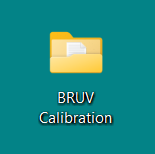
\includegraphics[keepaspectratio]{images/clipboard-2973557940.png}}
\item
  Dentro desta pasta, crie novos diretório (multiplas pastas) para cada
  configuração de BRUV. Estas distinções se baseiam principalmente na
  resolução da câmera utilizada e no campo de visão (\emph{Field of
  View}).
\end{enumerate}

\pandocbounded{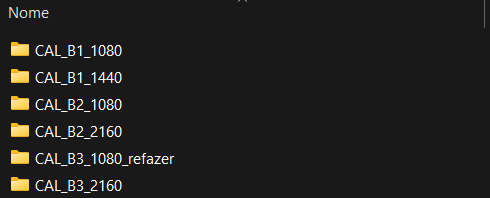
\includegraphics[keepaspectratio]{images/clipboard-387526838.png}}

\begin{enumerate}
\def\labelenumi{\arabic{enumi}.}
\setcounter{enumi}{2}
\item
  Dentro das respectivas pastas de BRUV, \textbf{cole} os respectivos os
  arquivos de vídeo (\textbf{.MP4}). Lembre-se, serão dois, um da câmera
  esquerda (E) e outro da câmera direita (D).

  \pandocbounded{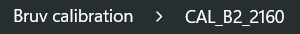
\includegraphics[keepaspectratio]{images/clipboard-2873460924.png}}

  \pandocbounded{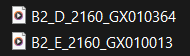
\includegraphics[keepaspectratio]{images/clipboard-328657837.png}}
\end{enumerate}

\begin{tcolorbox}[enhanced jigsaw, opacityback=0, toprule=.15mm, colframe=quarto-callout-tip-color-frame, arc=.35mm, breakable, rightrule=.15mm, left=2mm, leftrule=.75mm, colback=white, bottomrule=.15mm]
\begin{minipage}[t]{5.5mm}
\textcolor{quarto-callout-tip-color}{\faLightbulb}
\end{minipage}%
\begin{minipage}[t]{\textwidth - 5.5mm}

Para facilitar, \textbf{renomei} os arquivos de vídeo (.MP4) conforme a
\textbf{ID do BRUV}, o \textbf{lado da câmera} e a \textbf{resolução}
utilizada, seguindo nescessáriamente esta ordem. Ao final,
\textbf{mantenha o nome do arquivo original} gerado pela câmera. Não
utilize espaços nem caracteres especiais.

Ex: B2\_D\_2160\_GX010364 (\emph{bruvID\_lado\_resolucao\_nome
original}).

\end{minipage}%
\end{tcolorbox}

\begin{enumerate}
\def\labelenumi{\arabic{enumi}.}
\setcounter{enumi}{3}
\item
  Na mesma pasta de trabalho, adicione também a \textbf{cópia} do
  arquivo de calibração do cubo (\textbf{.PtsCAL}).

  \pandocbounded{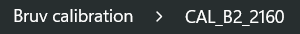
\includegraphics[keepaspectratio]{images/clipboard-1271673136.png}}

  \pandocbounded{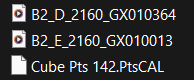
\includegraphics[keepaspectratio]{images/clipboard-3344884228.png}}
\end{enumerate}

\begin{tcolorbox}[enhanced jigsaw, opacityback=0, toprule=.15mm, colframe=quarto-callout-caution-color-frame, arc=.35mm, breakable, rightrule=.15mm, left=2mm, leftrule=.75mm, colback=white, bottomrule=.15mm]
\begin{minipage}[t]{5.5mm}
\textcolor{quarto-callout-caution-color}{\faFire}
\end{minipage}%
\begin{minipage}[t]{\textwidth - 5.5mm}

O arquivo de calibração do cubo (\textbf{.PtsCAL}) variam de acordo com
o modelo de cubo de calibração utilizado. Estes arquivos são fornecidos
pela SeaGIS no momento da compra. Se necessário, contacte a
representação da empresa.

\end{minipage}%
\end{tcolorbox}

\begin{enumerate}
\def\labelenumi{\arabic{enumi}.}
\setcounter{enumi}{4}
\item
  Além disso, adicione o arquivo de parâmetros da câmera
  (\textbf{.CamCAL}), conforme modelo e configuração empregada. Estes
  arquivos são fornecidos pela SeaGIS, no site:
  \url{https://www.seagis.com.au/download.php}.

  \pandocbounded{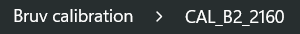
\includegraphics[keepaspectratio]{images/clipboard-1271673136.png}}

  \pandocbounded{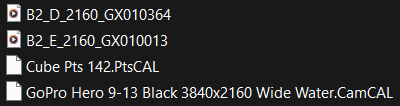
\includegraphics[keepaspectratio]{images/clipboard-742698619.png}}
\item
  Ao final, você terá, normalmente, 04 (quatro) arquivos:
\end{enumerate}

\begin{verbatim}
-   Vídeo da Câmera Esquerda (.MP4);

-   Vídeo da Câmera Direita (.MP4);

-   Arquivo de calibração do cubo (.PtsCAL), conforme modelo.

-   Arquivo de parâmetros da câmera (.CamCAL), conforme modelo e resolução.
\end{verbatim}

\begin{enumerate}
\def\labelenumi{\arabic{enumi}.}
\setcounter{enumi}{6}
\item
  Com o PEN-DRIVE fornecido pela SeaGIS conectado ao seu computador,
  inicie o programa de calibração CAL (Downloads:
  \url{https://www.seagis.com.au/download.php})
\item
  No CAL, crie um novo projeto através do menu: \emph{Project \textbar{}
  New project}

  \pandocbounded{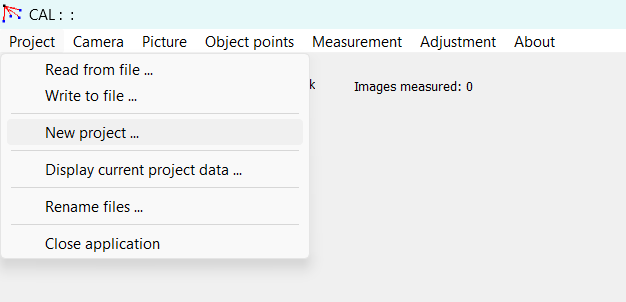
\includegraphics[keepaspectratio]{images/clipboard-3423544538.png}}
\item
  Você será solicitado para salvar quaisquer dados não salvos associados
  ao projeto atual. Insira um nome para o arquivo do projeto (por
  exemplo, \textbf{``\textbf{\emph{ProjCAL\_B2\_2160}}''}) e salve o
  arquivo do projeto no diretório que você acabou de criar para este
  projeto.
\end{enumerate}

\begin{verbatim}
![](images/clipboard-1271673136.png)

![](images/clipboard-3448108106.png)

::: {.callout-note appearance="simple"}
A criação de um novo projeto inicia um processo de assistente do próprio programa que irá solicitar a configuração do restante do projeto. Basta seguir as instruções, lembrando que todos os arquivos estão localizados no mesmo diretório, e que o CAL usará, por padrão, o diretório onde o novo arquivo de projeto foi criado.
:::
\end{verbatim}

\begin{enumerate}
\def\labelenumi{\arabic{enumi}.}
\setcounter{enumi}{9}
\item
  Carregue os arquivos de parâmetro da câmera esquerda e direita
  (\textbf{.CamCAL}), conforme solicitado.

  \begin{tcolorbox}[enhanced jigsaw, opacityback=0, toprule=.15mm, colframe=quarto-callout-caution-color-frame, arc=.35mm, breakable, rightrule=.15mm, left=2mm, leftrule=.75mm, colback=white, bottomrule=.15mm]
  \begin{minipage}[t]{5.5mm}
  \textcolor{quarto-callout-caution-color}{\faFire}
  \end{minipage}%
  \begin{minipage}[t]{\textwidth - 5.5mm}

  Atenção! É um mesmo arquivo (\textbf{.CamCAL}) para ambas as câmeras,
  pois utilizamos em cada lado do BRUV câmeras de mesmo modelo e mesma
  configuração.

  \end{minipage}%
  \end{tcolorbox}
\item
  Carregue o arquivo do cubo de calibração (\textbf{.PtsCAL}), conforme
  solicitado.
\item
  Defina o diretório de imagens conforme solicitado.

  \begin{tcolorbox}[enhanced jigsaw, opacityback=0, toprule=.15mm, colframe=quarto-callout-note-color-frame, arc=.35mm, breakable, rightrule=.15mm, left=2mm, leftrule=.75mm, colback=white, bottomrule=.15mm]
  \begin{minipage}[t]{5.5mm}
  \textcolor{quarto-callout-note-color}{\faInfo}
  \end{minipage}%
  \begin{minipage}[t]{\textwidth - 5.5mm}

  \textbf{O diretório de imagens é automaticamente definido como o mesmo
  diretório do arquivo do projeto}; portanto, se todos os arquivos da
  calibração estiverem em um único diretório, basta verificar e clicar
  em \textbf{OK}.

  \end{minipage}%
  \end{tcolorbox}
\item
  O programe pedirá para que salve o novo arquivo de medições
  (\textbf{.ObsCAL}) que será atrelado ao projeto. \textbf{Basta
  atribuir um nome a esse arquivo} (por exemplo,
  \textbf{``\textbf{\emph{MeasureCAL\_B2\_2160}}''}). Este arquivo será
  o local onde as medições da calibração serão armazenadas.

  \begin{tcolorbox}[enhanced jigsaw, opacityback=0, toprule=.15mm, colframe=quarto-callout-note-color-frame, arc=.35mm, breakable, rightrule=.15mm, left=2mm, leftrule=.75mm, colback=white, bottomrule=.15mm]
  \begin{minipage}[t]{5.5mm}
  \textcolor{quarto-callout-note-color}{\faInfo}
  \end{minipage}%
  \begin{minipage}[t]{\textwidth - 5.5mm}

  O programa também irá gerar um arquivo de \emph{backup} automático das
  medições (\textbf{.ObsCAL\_AUTO}).

  \end{minipage}%
  \end{tcolorbox}

  \pandocbounded{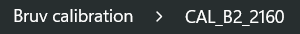
\includegraphics[keepaspectratio]{images/clipboard-1271673136.png}}

  \pandocbounded{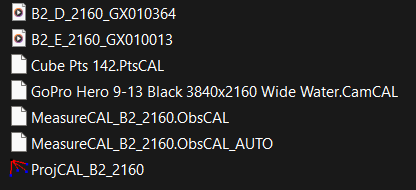
\includegraphics[keepaspectratio]{images/clipboard-3041673086.png}}
\item
  Carregue o arquivo de vídeo da câmera \textbf{ESQUERDA}. Ele será
  automaticamente adicionado à configuração da sequência de filmes. Caso
  existam mais arquivos de vídeo na sequência, eles podem ser
  adicionados nesse momento (ver \textbf{Sequências de filmes}). Em
  seguida, clique em \textbf{OK}.
\item
  Carregue o arquivo de vídeo da câmera \textbf{DIREITA}. Idem.
\item
  A janela \emph{Current project files} (\emph{Arquivos do projeto
  atual}) será exibida. \textbf{Todos os campos devem estar preenchidos}
  e todos os itens listados devem estar no \textbf{mesmo diretório}.
  Clique em \emph{Close dialog} (\emph{Fechar diálogo}).

  \pandocbounded{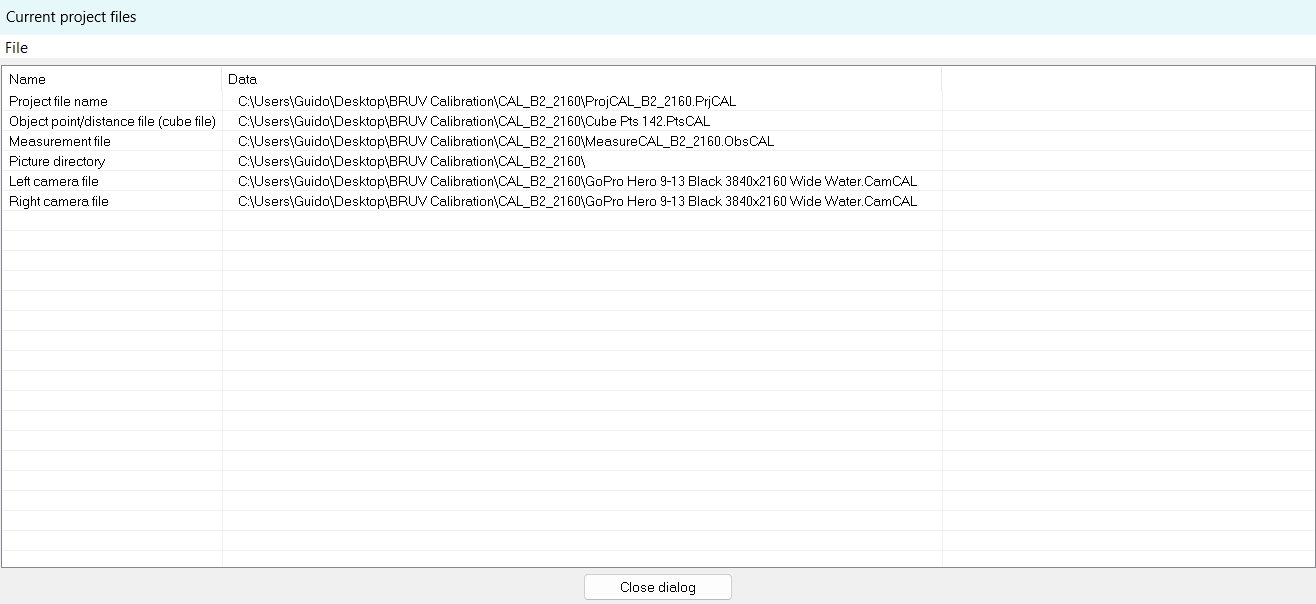
\includegraphics[keepaspectratio]{images/clipboard-3162917403.png}}
\end{enumerate}

\section{Explore mais!}\label{explore-mais}

\begin{itemize}
\item
  Se for em \emph{Camera \textbar{} Left/Right \textbar{} Edit
  parameters}, você terá acesso as características ópticas da câmera.

  \pandocbounded{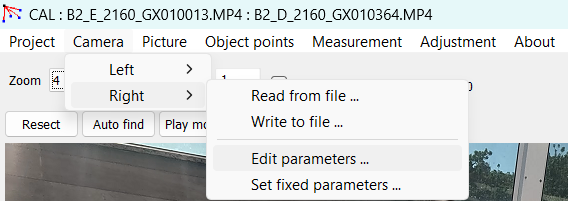
\includegraphics[keepaspectratio]{images/clipboard-175649103.png}}
\item
  Essas informações são importantes quando se trabalha cientificamente
  com a visão.

  \pandocbounded{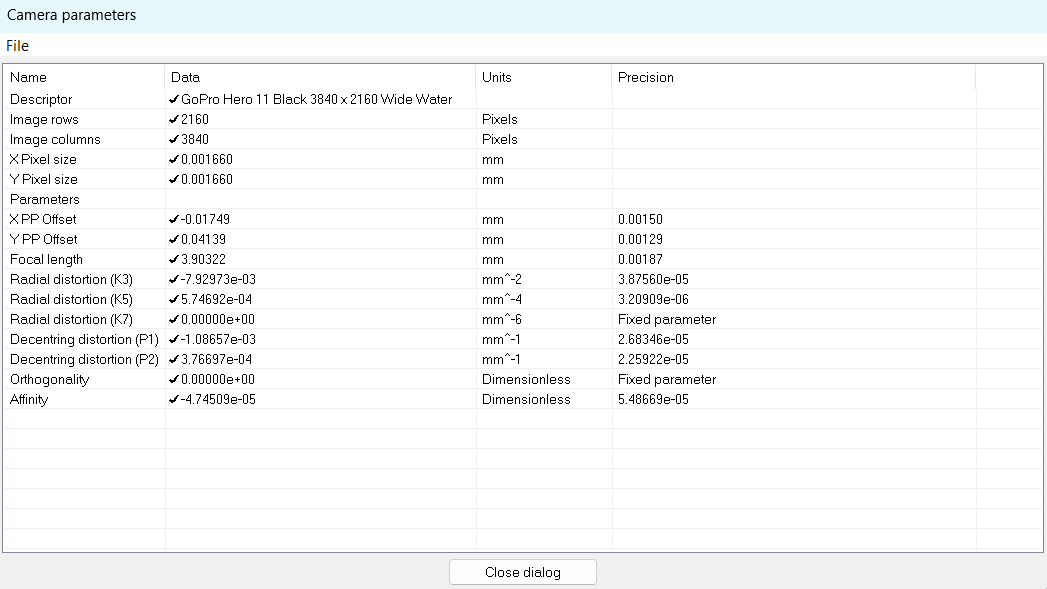
\includegraphics[keepaspectratio]{images/clipboard-1832882555.png}}
\item
  É importante sempre anotar a versão do programa. Essas informações
  devem constar na seção de métodos de possíveis manuscritos acadêmicos,
  pois representam o estado exato dos algorítimos utilizados nos
  cálculos realizados pelo programa.
\end{itemize}

\section{Sincronizando Câmeras}\label{sincronizando-cuxe2meras}

\begin{enumerate}
\def\labelenumi{\arabic{enumi}.}
\item
  Plug o pen-drive no USB.
\item
  Abra o programa CAL no seu computador (Downloads:
  \url{https://www.seagis.com.au/download.php})
\end{enumerate}

\pandocbounded{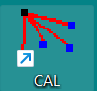
\includegraphics[keepaspectratio]{images/clipboard-316596302.png}}

\begin{enumerate}
\def\labelenumi{\arabic{enumi}.}
\setcounter{enumi}{2}
\item
  Se você já tinha um projeto salvo, o programa abrirá automaticamente
  nele. Ele sempre reinicia no último projeto que você trabalhou.

  \begin{tcolorbox}[enhanced jigsaw, opacityback=0, toprule=.15mm, colframe=quarto-callout-note-color-frame, arc=.35mm, breakable, rightrule=.15mm, left=2mm, leftrule=.75mm, colback=white, bottomrule=.15mm]
  \begin{minipage}[t]{5.5mm}
  \textcolor{quarto-callout-note-color}{\faInfo}
  \end{minipage}%
  \begin{minipage}[t]{\textwidth - 5.5mm}

  Acho que dá para mudar isso nas configurações, é bom rever manual!

  \end{minipage}%
  \end{tcolorbox}
\item
  Agora a gente vai sincronizar a câmera. Para isso clique em \emph{Play
  movie} na câmera \textbf{esquerda}

  \pandocbounded{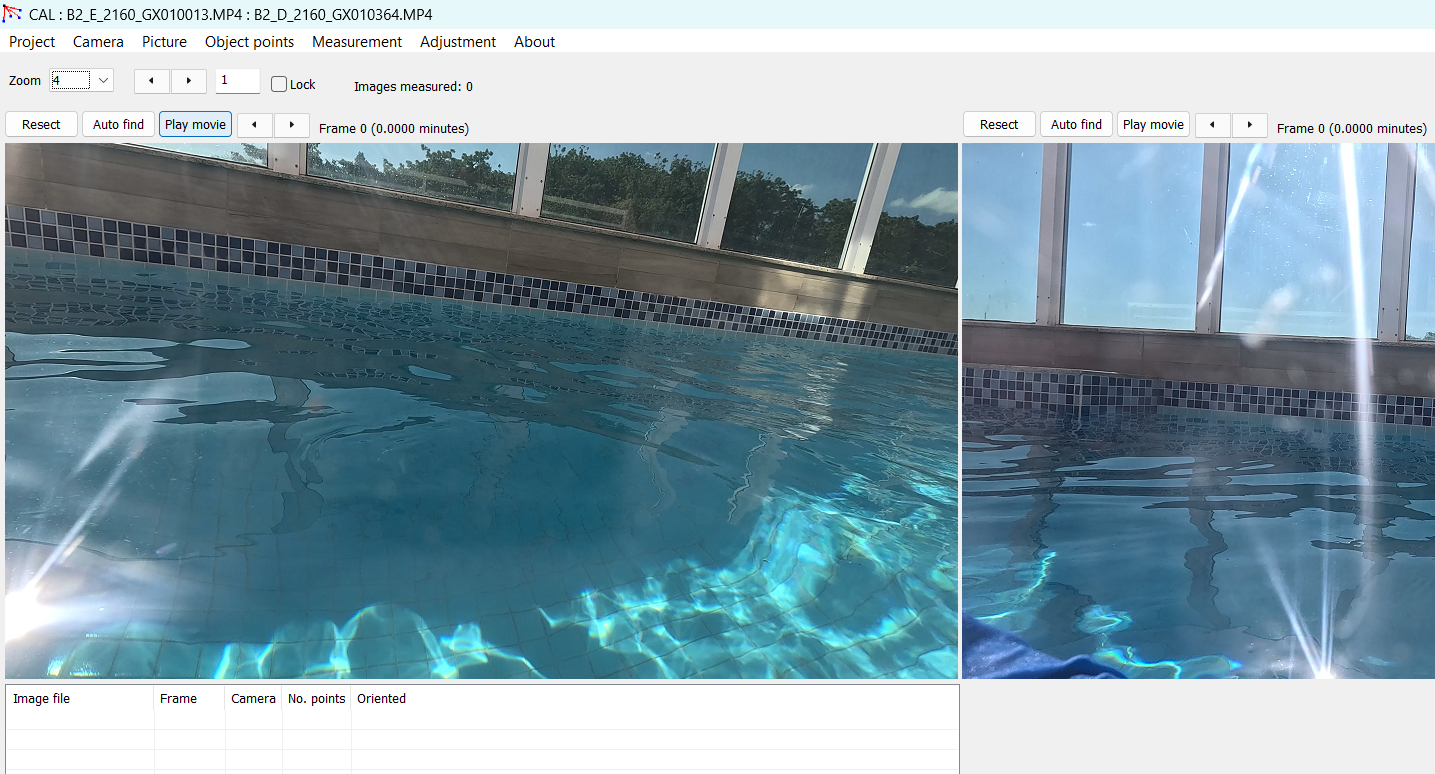
\includegraphics[keepaspectratio]{images/clipboard-1011136995.png}}
\item
  É para esse momento que serve o bater palmas ou os dedos (movimentos
  de \emph{clap}). Servindo de claquete para marcar o início da tomada,
  para gerarmos oo sincronismo audiovisual entre imagem e som.

  \begin{tcolorbox}[enhanced jigsaw, opacityback=0, toprule=.15mm, colframe=quarto-callout-warning-color-frame, arc=.35mm, breakable, rightrule=.15mm, left=2mm, leftrule=.75mm, colback=white, bottomrule=.15mm]
  \begin{minipage}[t]{5.5mm}
  \textcolor{quarto-callout-warning-color}{\faExclamationTriangle}
  \end{minipage}%
  \begin{minipage}[t]{\textwidth - 5.5mm}

  ATENÇÃO, AVISO DAS GALÁXIAS!

  NUNCA ESQUEÇA DE REALIZAR O ``CLAP'' ANTES DE LANÇAR OS BRUVS!

  Trata-se de um esquecimento comum durante as operações de campo, pois
  a dinâmica da atividade embarcada associada a um conjunto de passos
  que precisam ser seguidos antes do lançamento, nos leva a esquecer dos
  procedimentos mais simples.

  A realização dessa operação é fundamental para a sincronização
  posterior das câmeras dentro do programa de fotogrametria, seja para
  tomada de medida ou na etapa de calibração.

  A não realização ou esquecimento dessa etapa pode inviabilizar toda a
  amostragem do dia, desperdiçando assim nosso esforço de campo,
  financeiro e físico.

  Ainda que possível realizar a sincronização na ausência deste
  movimento, a operação será muito mais trabalhosa, despedindo muito
  mais capricho e tempo para a realização de uma simple etapa.

  Atente-se que por se tratar de um sistema de \textbf{stereo}-BRUV, com
  \textbf{câmeras em diferentes ângulos}, você pode acabar obstruindo a
  visualização de uma delas a depender da sua posição em relação a elas.

  \textbf{Se faz necessário que ambas as câmeras registre o movimento
  ``clap''.}

  \end{minipage}%
  \end{tcolorbox}

  \begin{tcolorbox}[enhanced jigsaw, opacityback=0, toprule=.15mm, colframe=quarto-callout-tip-color-frame, arc=.35mm, breakable, rightrule=.15mm, left=2mm, leftrule=.75mm, colback=white, bottomrule=.15mm]
  \begin{minipage}[t]{5.5mm}
  \textcolor{quarto-callout-tip-color}{\faLightbulb}
  \end{minipage}%
  \begin{minipage}[t]{\textwidth - 5.5mm}

  \textbf{A dica é utilizar movimentos rápidos e precisos.}

  \textbf{Sugiro o movimento de pinçar os dedos, como um caranguejo,
  batendo de forma rápida o polegar contra o indicador várias vezes
  seguidas de modo a aumentarmos a chance de captura limpa.}

  \end{minipage}%
  \end{tcolorbox}
\item
  Uma nova tela abrirá:

  \pandocbounded{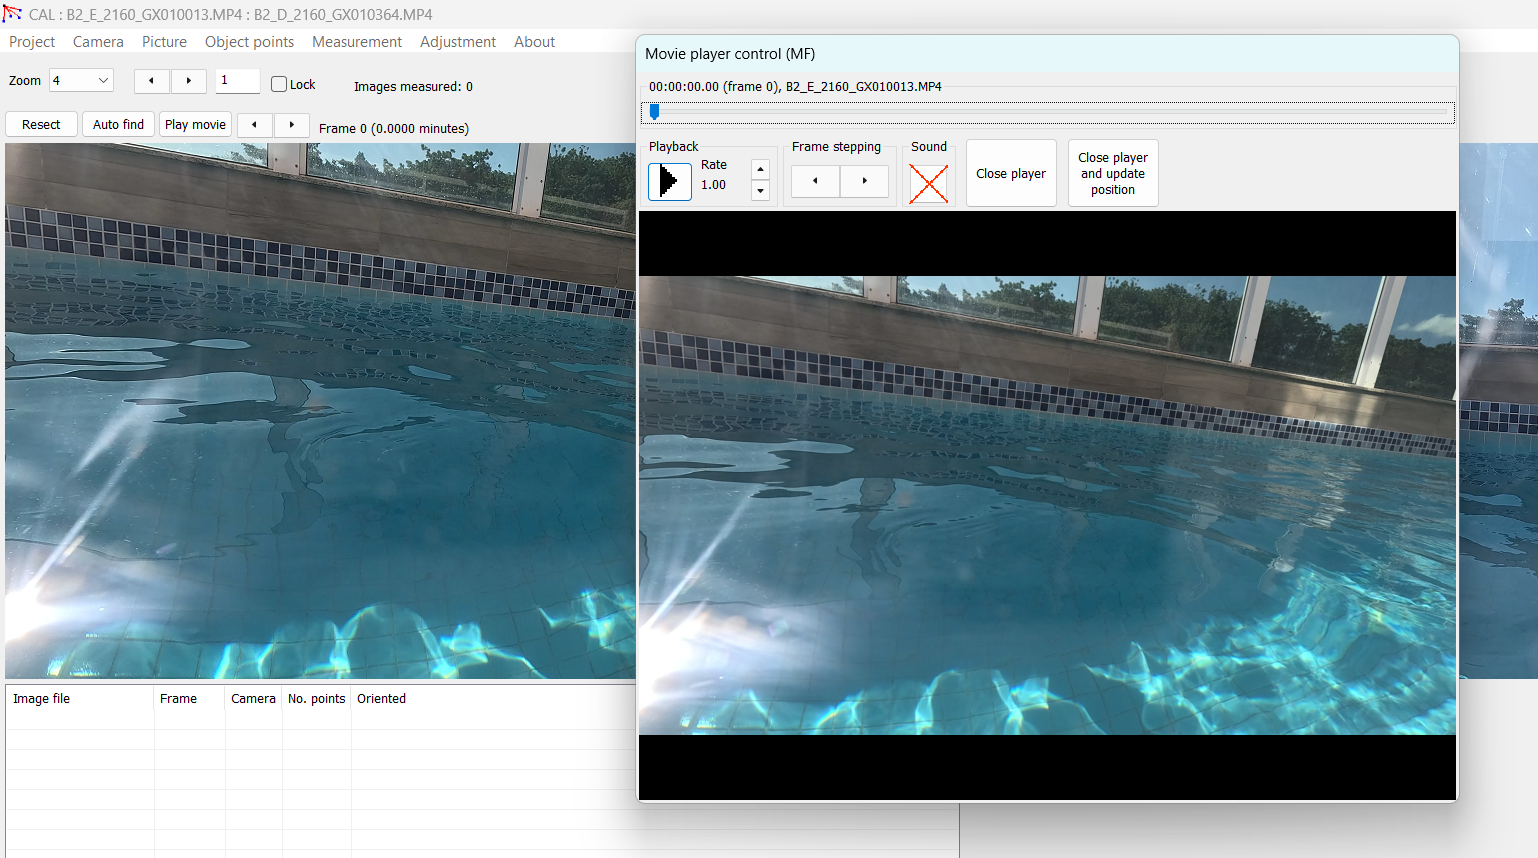
\includegraphics[keepaspectratio]{images/clipboard-1263872465.png}}
\item
  Aumente o \emph{Rate} para 5 (ou mude de acordo com a distância).

  \pandocbounded{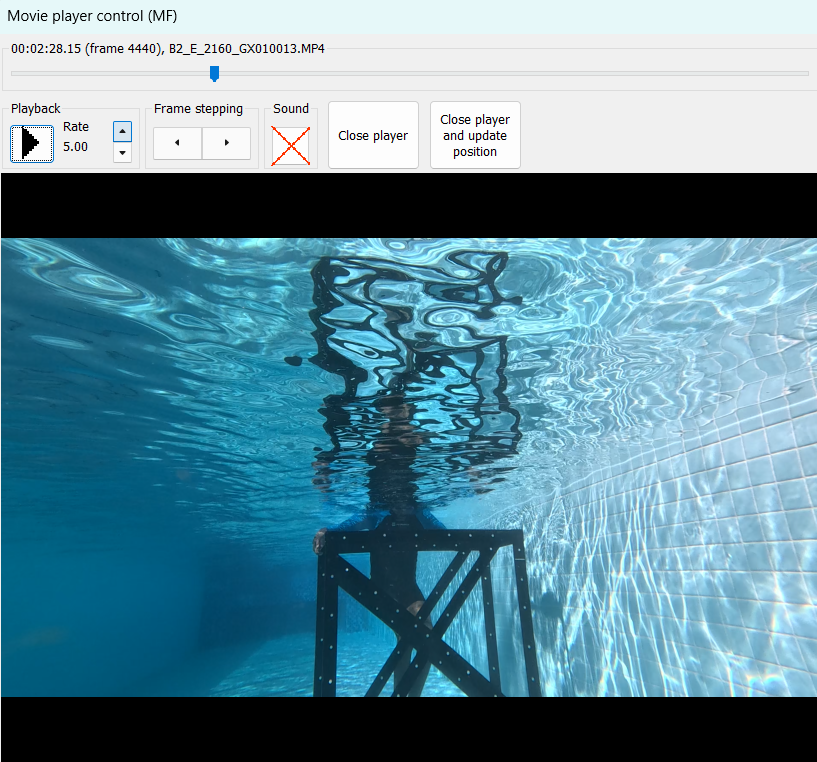
\includegraphics[keepaspectratio]{images/clipboard-2924529957.png}}
\item
  Aperte \emph{Playback} ▶️
\item
  Agora busque o momento sublime do \emph{clap} (ou \emph{clap clap}).

  \begin{tcolorbox}[enhanced jigsaw, opacityback=0, toprule=.15mm, colframe=quarto-callout-tip-color-frame, arc=.35mm, breakable, rightrule=.15mm, left=2mm, leftrule=.75mm, colback=white, bottomrule=.15mm]
  \begin{minipage}[t]{5.5mm}
  \textcolor{quarto-callout-tip-color}{\faLightbulb}
  \end{minipage}%
  \begin{minipage}[t]{\textwidth - 5.5mm}

  Não use a barra de rolagem do vídeo. Até dá para usar de forma
  grosseira para tentar chegar o mais perto do momento clap. Assim, que
  você tentar, verá que ela não tem movimentos preciso e atrapalha mais
  do que ajuda.

  \end{minipage}%
  \end{tcolorbox}
\item
  Quando passar ou estiver próximo, \emph{Pause!}
\item
  Use o \emph{Frame stepping} para avançar ou retroceder no momento
  antecessor ao \emph{clap}.

  \pandocbounded{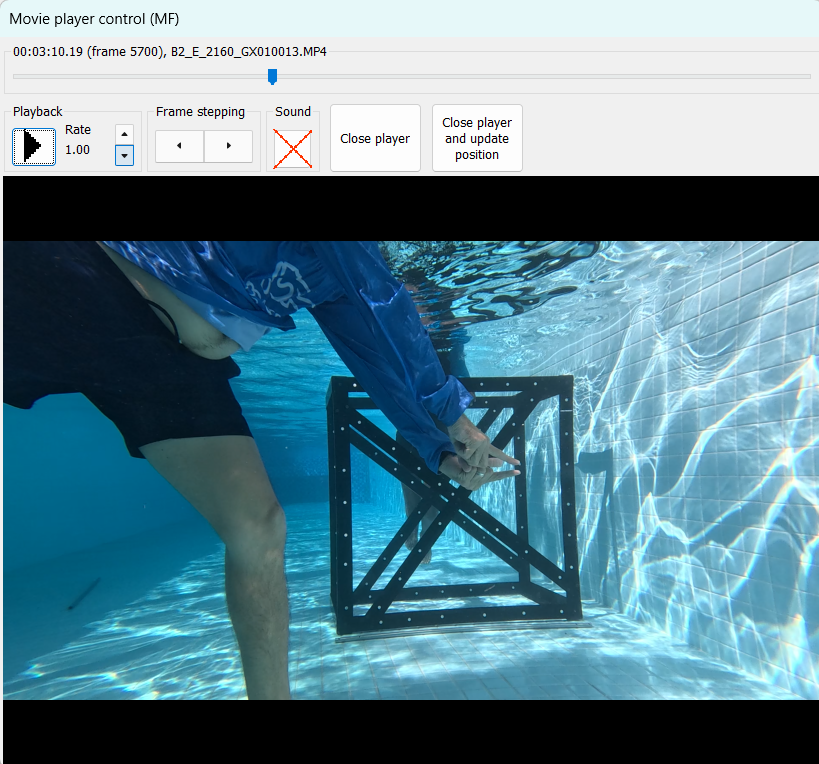
\includegraphics[keepaspectratio]{images/clipboard-10482523.png}}
\item
  Agora reduza o \emph{Rate} para 1 e vá avançando no \emph{Frame
  stepping} até o momento \emph{clap} e clique em \emph{Close player and
  update position}.

  \pandocbounded{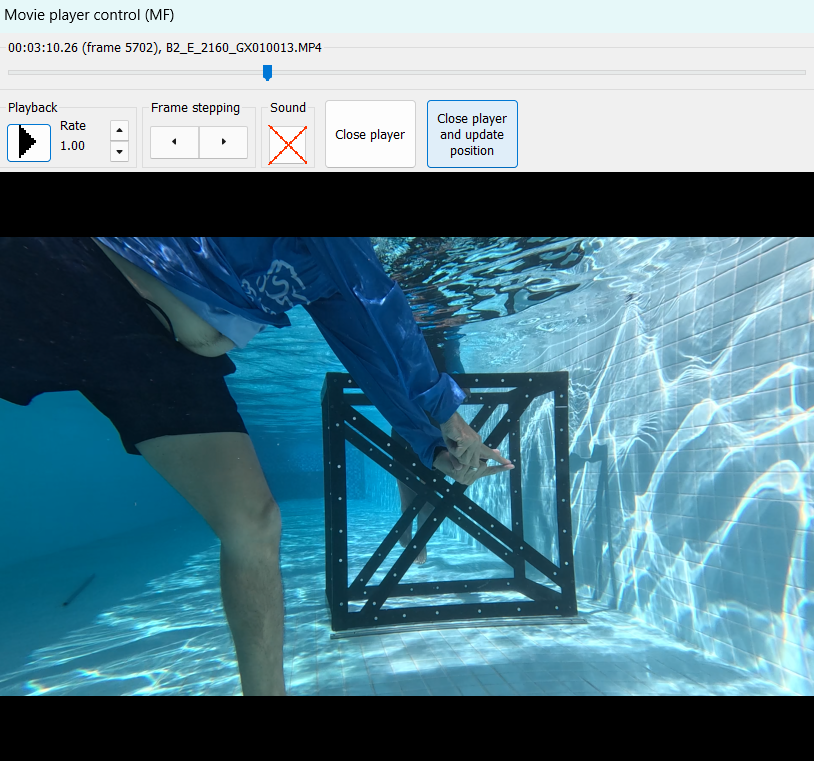
\includegraphics[keepaspectratio]{images/clipboard-3408781496.png}}
\item
  Agora faça o mesmo para a câmera da direita. Aperte \emph{Play movie}.

  \pandocbounded{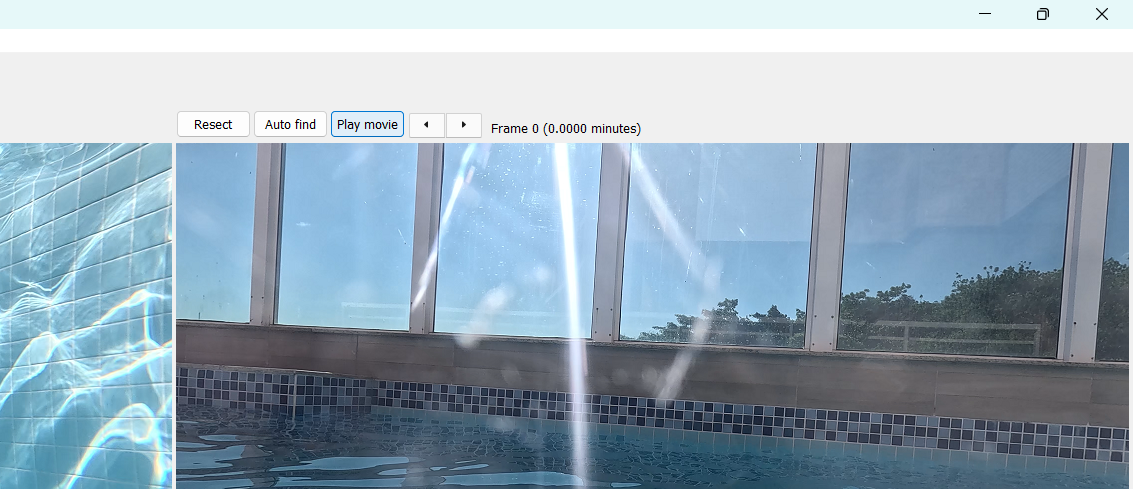
\includegraphics[keepaspectratio]{images/clipboard-1804368135.png}}
\item
  Encontre o momento \emph{clap} e cliquei em \emph{Close player and
  update position}

  \pandocbounded{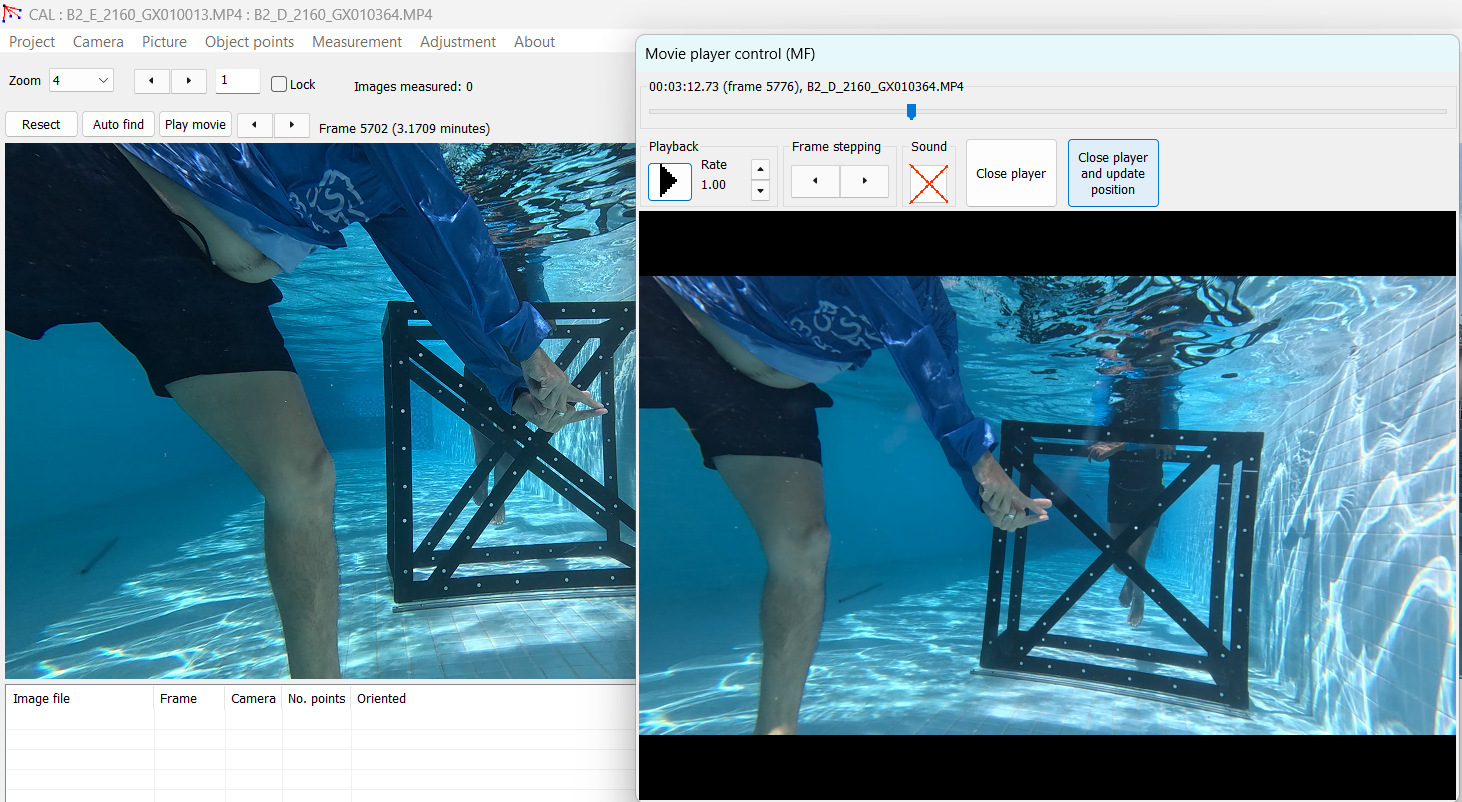
\includegraphics[keepaspectratio]{images/clipboard-3998749045.png}}
\item
  Agora sim, começaremos os trabalhos.
\item
  Ative o botão \emph{Lock}

  \pandocbounded{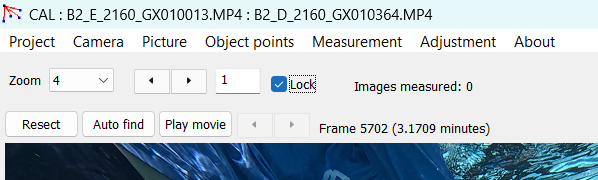
\includegraphics[keepaspectratio]{images/clipboard-3929359159.png}}
\item
  Aperte \emph{Play movie} na câmera esquerda, abrirá a janela do
  \emph{Movie player control}. Aumente o \emph{Rate} (ex: 3) e clique em
  \emph{Playback} ▶️. Pause no momento que antecede os movimentos
  sequenciais (são 20 ao todo) que o quadrado de calibração precisa
  fazer para calibrar (Ver manual).

  \pandocbounded{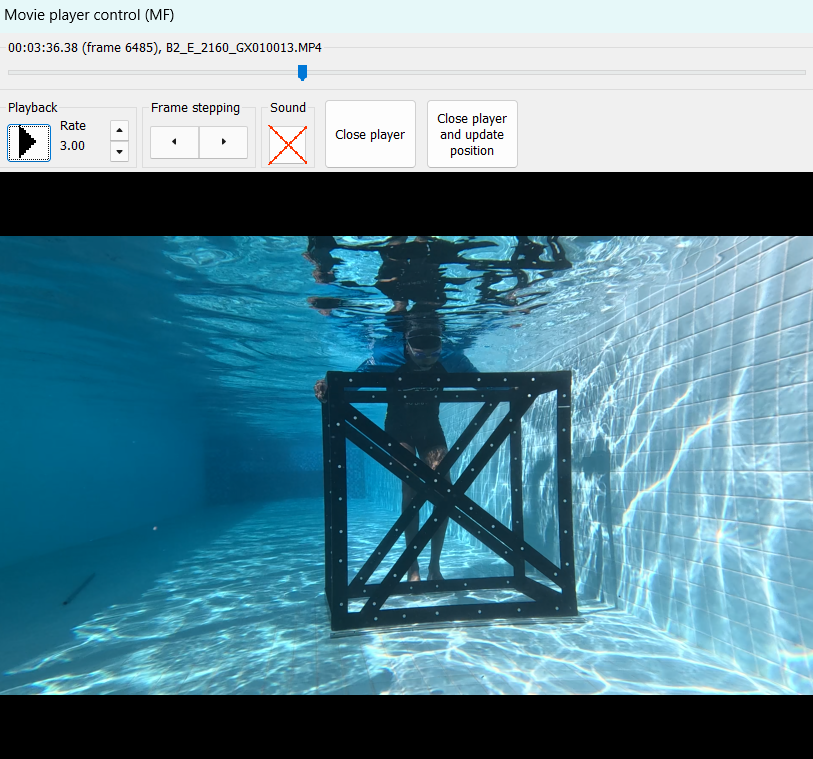
\includegraphics[keepaspectratio]{images/clipboard-2925575631.png}}

  \begin{tcolorbox}[enhanced jigsaw, opacityback=0, toprule=.15mm, colframe=quarto-callout-caution-color-frame, arc=.35mm, breakable, rightrule=.15mm, left=2mm, leftrule=.75mm, colback=white, bottomrule=.15mm]
  \begin{minipage}[t]{5.5mm}
  \textcolor{quarto-callout-caution-color}{\faFire}
  \end{minipage}%
  \begin{minipage}[t]{\textwidth - 5.5mm}

  Perceba que na situação ilustrativa acima, o quadro de calibração se
  encontra relativamente distante em relação as câmeras. É preciso
  buscar um melhor enquadramento.

  \end{minipage}%
  \end{tcolorbox}
\item
  Aperte \emph{Close player and update position} e perceba que ambas as
  câmeras irão atualizar para o frame em questão. Isso se deve por
  termos selecionado o botão \emph{Lock}.
\end{enumerate}

\section{Começando os trabalhos}\label{comeuxe7ando-os-trabalhos}

\begin{enumerate}
\def\labelenumi{\arabic{enumi}.}
\item
  Agora, vamos começar marcar os pontos. Comece pelo frame da câmera
  esquerda. Este processo precisara se feitos em ambas as câmeras (02)
  para cada sequência de frame (20), no mínimo (20*2=40), seguindo o
  esquema de ponto, \textbf{conforme o modelo do seu cubo de calibração}
  (Ex: Cubo 142, abaixo):

  \pandocbounded{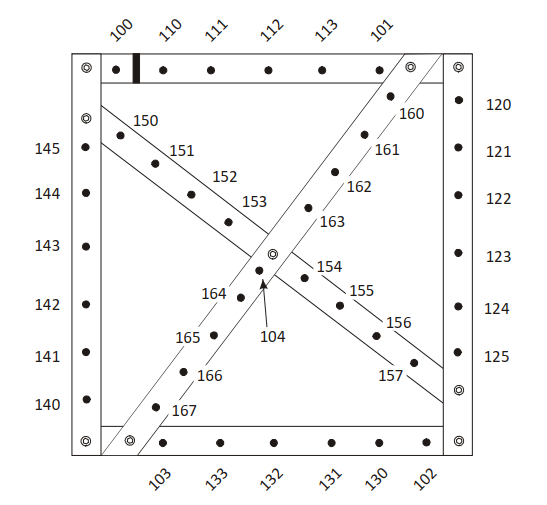
\includegraphics[keepaspectratio]{images/clipboard-2197934981.png}}
\item
  Começe pelo ponto 100, que enontra-se justo acima da linha de
  referência. Depois siga para o 101, 102, 103 e 104, estes são os
  \textbf{pontos de} \footnote{Ressecção: É uma processo/ técnica da
    visão computacional e fotogrametria utilizada para determinar a
    posição e orientação da câmera no espaço a partir de pontos
    conhecidos no mundo (objeto).} (\emph{ressection points}). A partir
  daí, 110 em diante. Você perceberar que essa sequência já está pre
  programada dentro do programa.

  \begin{tcolorbox}[enhanced jigsaw, opacityback=0, toprule=.15mm, colframe=quarto-callout-tip-color-frame, arc=.35mm, breakable, rightrule=.15mm, left=2mm, leftrule=.75mm, colback=white, bottomrule=.15mm]
  \begin{minipage}[t]{5.5mm}
  \textcolor{quarto-callout-tip-color}{\faLightbulb}
  \end{minipage}%
  \begin{minipage}[t]{\textwidth - 5.5mm}

  Utilize o material de apoio que eleboramos para você não se perder,
  tanto na sequência do quadrado como na posição dos pontos (POR LINK).

  \end{minipage}%
  \end{tcolorbox}
\item
  Um dica é apertar \emph{Ctrl} no teclado e avançar com o mouse para
  frente, isso irá dar zoom.

  \pandocbounded{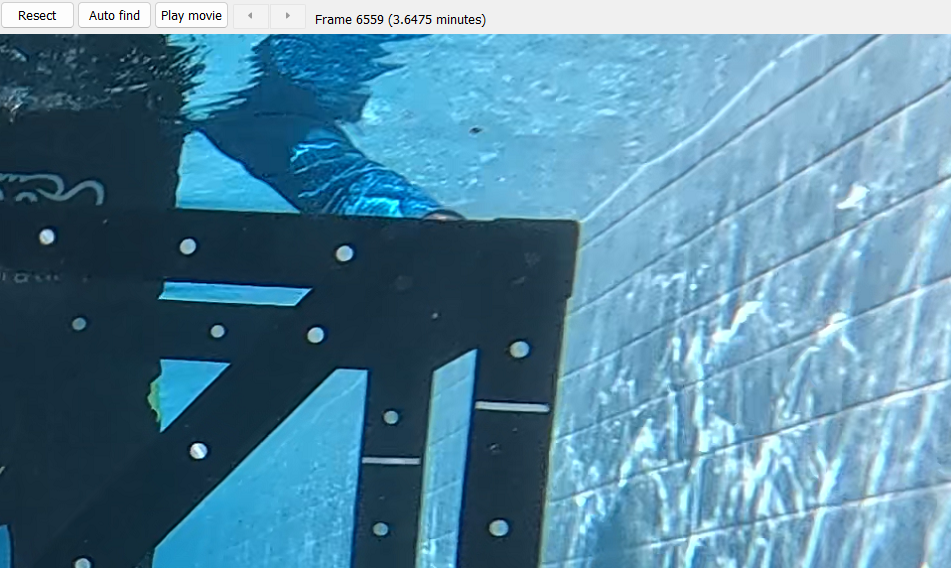
\includegraphics[keepaspectratio]{images/clipboard-308469490.png}}

  \begin{tcolorbox}[enhanced jigsaw, opacityback=0, toprule=.15mm, colframe=quarto-callout-warning-color-frame, arc=.35mm, breakable, rightrule=.15mm, left=2mm, leftrule=.75mm, colback=white, bottomrule=.15mm]
  \begin{minipage}[t]{5.5mm}
  \textcolor{quarto-callout-warning-color}{\faExclamationTriangle}
  \end{minipage}%
  \begin{minipage}[t]{\textwidth - 5.5mm}

  É, não dá para usar a bala de rolagem do mouse.

  \end{minipage}%
  \end{tcolorbox}
\item
  Aperte \emph{Shift} e um pequeno quadrado irá aparecer, este é o
  \textbf{Centroíde.}

  \pandocbounded{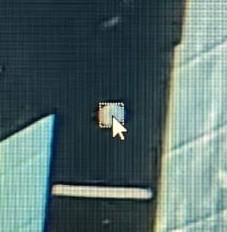
\includegraphics[keepaspectratio]{images/WhatsApp Image 2026-02-24 at 10.27.30.jpeg}}

  \begin{tcolorbox}[enhanced jigsaw, opacityback=0, toprule=.15mm, colframe=quarto-callout-note-color-frame, arc=.35mm, breakable, rightrule=.15mm, left=2mm, leftrule=.75mm, colback=white, bottomrule=.15mm]
  \begin{minipage}[t]{5.5mm}
  \textcolor{quarto-callout-note-color}{\faInfo}
  \end{minipage}%
  \begin{minipage}[t]{\textwidth - 5.5mm}

  O centróide serve como um alvo que facilita a realização da medida.
  Realizar a medida via centróide é 10x melhor do que realizar apenas
  clicando diretamente (\emph{point and click).}

  \end{minipage}%
  \end{tcolorbox}
\item
  Ainda com o \emph{Shift} pressionado, aponte a flecha do mouse no
  centro e clique com o botão esquerdo do mouse para marcar um ponto.

  \pandocbounded{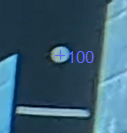
\includegraphics[keepaspectratio]{images/clipboard-3599675830.png}}
\item
  Marque os pontos ressecionáis (conforme já mencionado anteriormente).
\item
  Em um determinado momento o CAL irá tentar plotar os demais pontos
  automáticamente.

  \pandocbounded{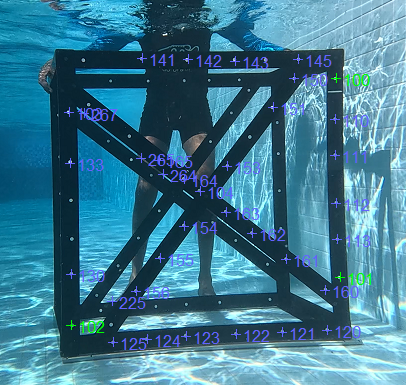
\includegraphics[keepaspectratio]{images/clipboard-444453288.png}}

  \begin{tcolorbox}[enhanced jigsaw, opacityback=0, toprule=.15mm, colframe=quarto-callout-note-color-frame, arc=.35mm, breakable, rightrule=.15mm, left=2mm, leftrule=.75mm, colback=white, bottomrule=.15mm]
  \begin{minipage}[t]{5.5mm}
  \textcolor{quarto-callout-note-color}{\faInfo}
  \end{minipage}%
  \begin{minipage}[t]{\textwidth - 5.5mm}

  Ele acertará muitos e errará outros tantos. Alguns ele não irá
  encontrar, em especial os do segundo plano (200, 201\ldots).
  Independente disso você terá que verificar e corrigir cada um deles
  pontualmente.

  \end{minipage}%
  \end{tcolorbox}
\item
  Pontos ressecionáis (100,101,102,103 e 104) verdes indicam que foram
  bem calibrados.

  \pandocbounded{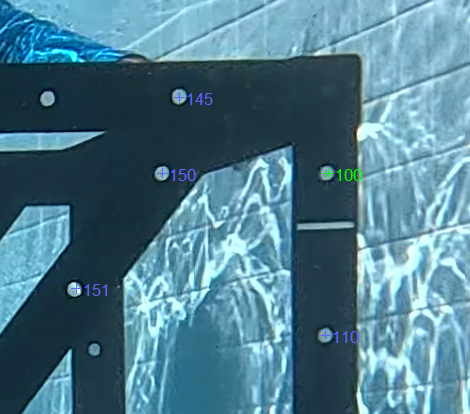
\includegraphics[keepaspectratio]{images/clipboard-1275978551.png}}
\item
  Quantos mais pontos verdes em cada frame, melhor!
\item
  Se o ponto gerado pelo CAL cair no lugar errado, delete.

  \pandocbounded{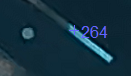
\includegraphics[keepaspectratio]{images/clipboard-1478588733.png}}
\item
  Ponha o cursor do mouse sobre o ponto e clique com o botão direito do
  mouse.

  \pandocbounded{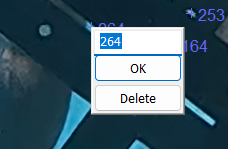
\includegraphics[keepaspectratio]{images/clipboard-1315559121.png}}
\item
  Plote você manualmente. Zoom in (Ctrl+mouse) \textgreater{}
  Centroiding (Shift) \textgreater{} Point (mouse esquerdo)
\item
  Provavelmente sairá outra numeração que não a correta.
  \pandocbounded{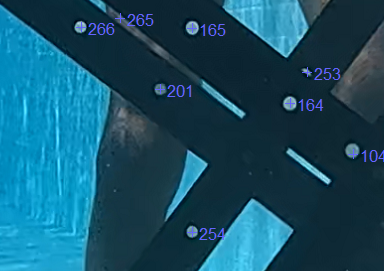
\includegraphics[keepaspectratio]{images/clipboard-3014583428.png}}
\item
  Clique com o botão direito do mouse sobre ele e renomei para a
  numeração que você achar que é. Aperte *OK*.

  \pandocbounded{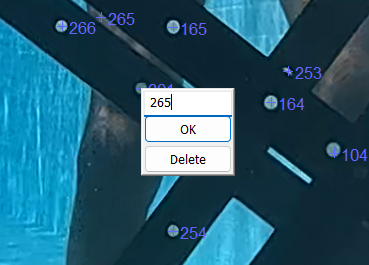
\includegraphics[keepaspectratio]{images/clipboard-3952036695.png}}
\item
  Tente encontrar o máximo de pontos que conseguir. As informações
  ficaram registradas abaixo da tela esquerda:

  \pandocbounded{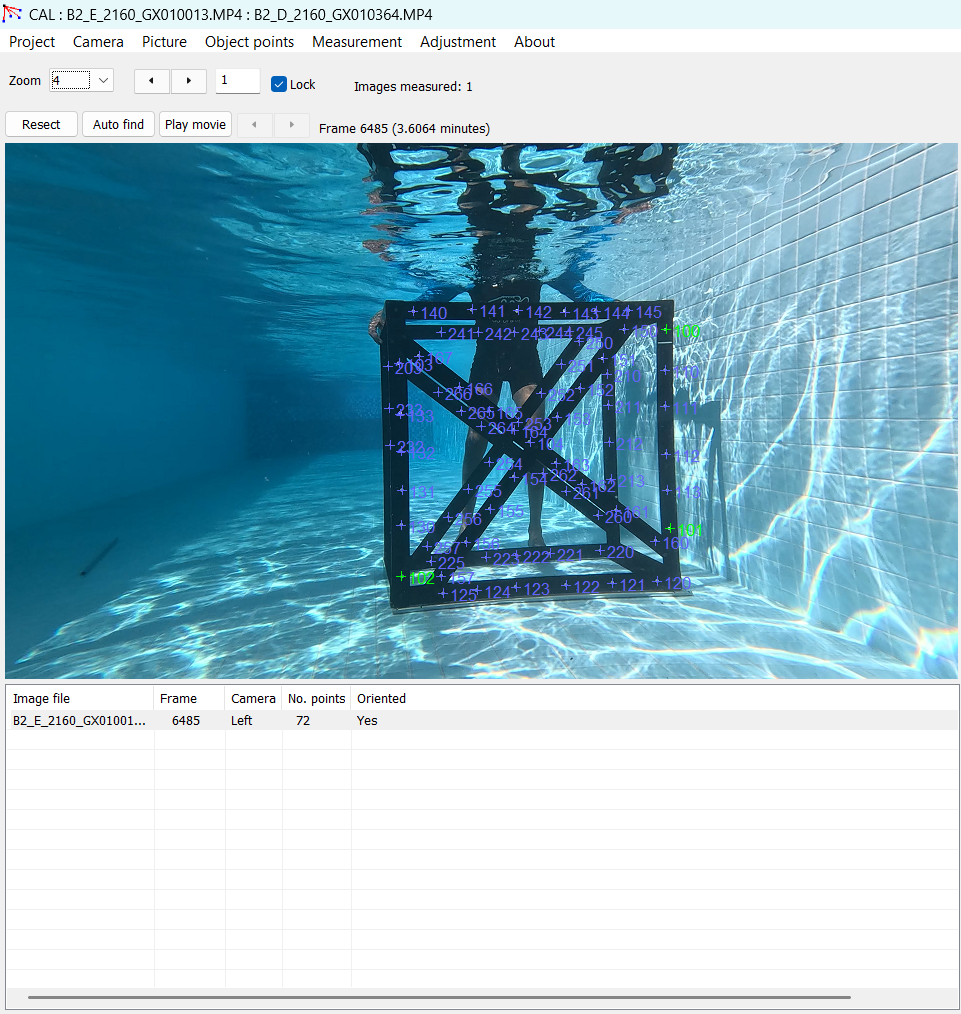
\includegraphics[keepaspectratio]{images/clipboard-1103650313.png}}
\item
  Quanto mais pontos (\emph{No.~points}) encontrar, mais preciso será a
  calibração, em teoria.
\end{enumerate}

\begin{verbatim}
::: {.callout-tip appearance="simple"}
Particurlamente, busco frames que me permitam acima de 70 pontos. Contudo, caso o frame em questão não atinja tal valor, siga com a calibração até o fim e caso não alcance uma boa precisão ao final, busque novos frames que permita acima de 70 ponto, para cada posição do cubo. 
:::
\end{verbatim}

\begin{enumerate}
\def\labelenumi{\arabic{enumi}.}
\setcounter{enumi}{16}
\item
  Pontos ressectíveis vermelhos é um mau sinal. Quanto maior o número
  deles pior.

  \pandocbounded{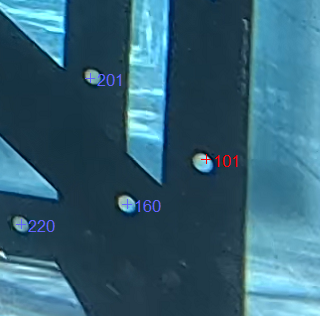
\includegraphics[keepaspectratio]{images/clipboard-2138859243.png}}
\item
  Após realizar a marcação de ambos os frames (Esquerda e Direita), siga
  para uma nova posição do cubo, conforme traz o manual de calibração:

  \pandocbounded{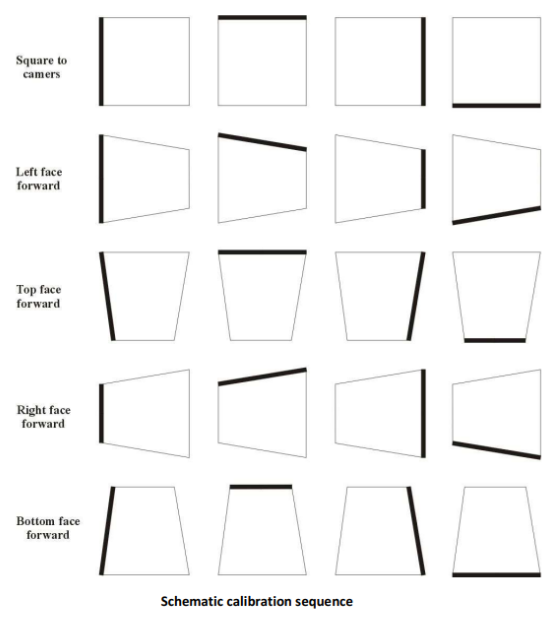
\includegraphics[keepaspectratio]{images/clipboard-2299725427.png}}
\item
  Para isso, aperte mais uma vez o botão \emph{Play movie} e a janela do
  \emph{Movie player control}, aperte \emph{Playback} ▶️ para o video
  seguir seu curso. Aperte \emph{Pause} quando o cubo estiver na próxima
  posição da sequência de calibração e aperte \emph{Close players and
  update position}.

  \begin{tcolorbox}[enhanced jigsaw, opacityback=0, toprule=.15mm, colframe=quarto-callout-important-color-frame, arc=.35mm, breakable, rightrule=.15mm, left=2mm, leftrule=.75mm, colback=white, bottomrule=.15mm]
  \begin{minipage}[t]{5.5mm}
  \textcolor{quarto-callout-important-color}{\faExclamation}
  \end{minipage}%
  \begin{minipage}[t]{\textwidth - 5.5mm}

  Pause no ângulo que maximize a exposição dos pontos do plano posterior
  (201, 202\ldots), evitando que as barras do primeiro plano se
  sobreponha as pontos do segundo plano. Contudo, em alguma das câmera
  sempre haverá algum ponto que será coberto.

  \end{minipage}%
  \end{tcolorbox}

  \pandocbounded{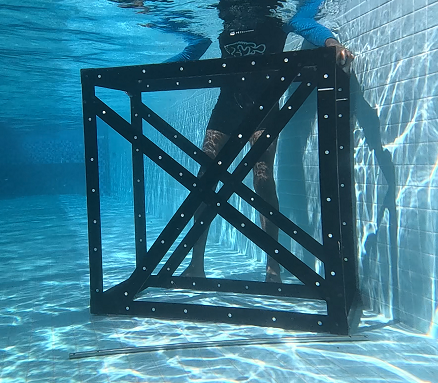
\includegraphics[keepaspectratio]{images/clipboard-2605035701.png}}\pandocbounded{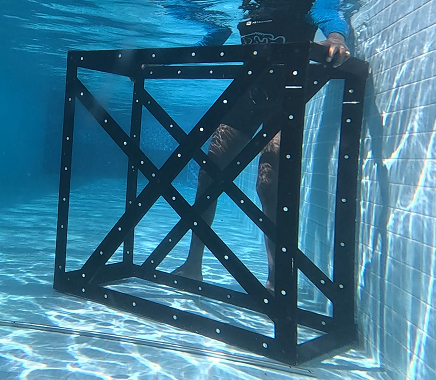
\includegraphics[keepaspectratio]{images/clipboard-3247803596.png}}
\item
  Remarque todos os pontos mais uma vez (Esquerda e Direita) e repita a
  operação para toda a sequência de posições do cubo. 😅
\item
  Um dica para não se perder no processo é ir marcando as posições do
  cubo que já foram realizadas, conforme abaixo:

  \pandocbounded{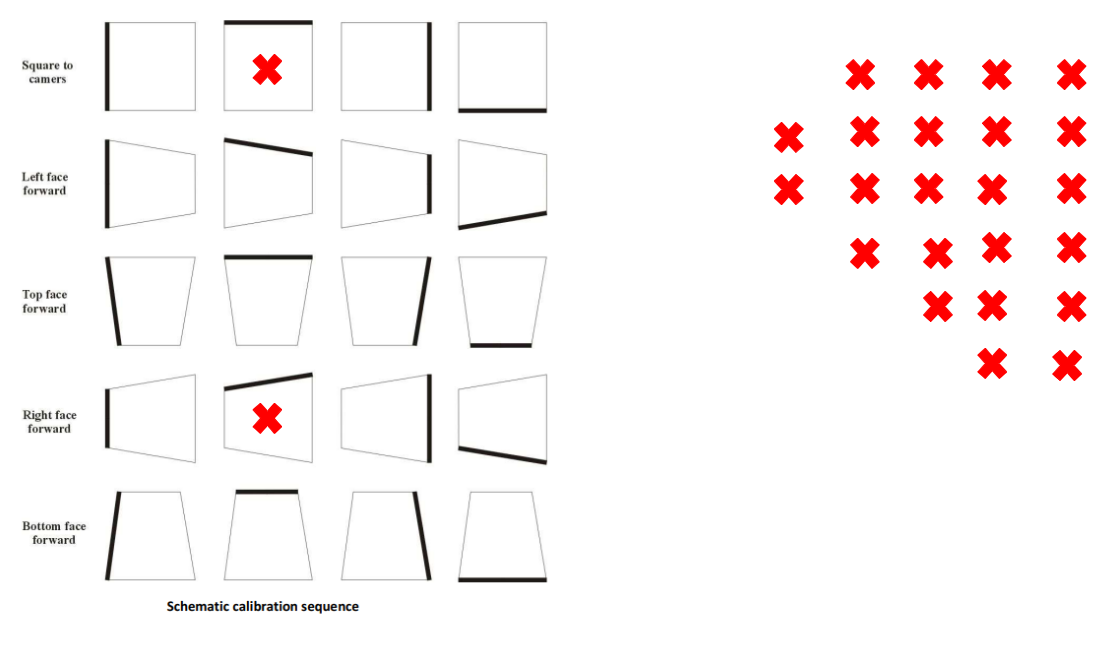
\includegraphics[keepaspectratio]{images/clipboard-44037176.png}}
\item
  Tenho esse arquivo (.ppt) disponível para ser compartilhado no drive
  do PMB.
\item
  As linhas pretas representam a linha branca de referência do cubo. Por
  exemplo, a imagem abaixo representa a quarta linha da segunda coluna
  do esquema de calibração ilustrado acima.

  \pandocbounded{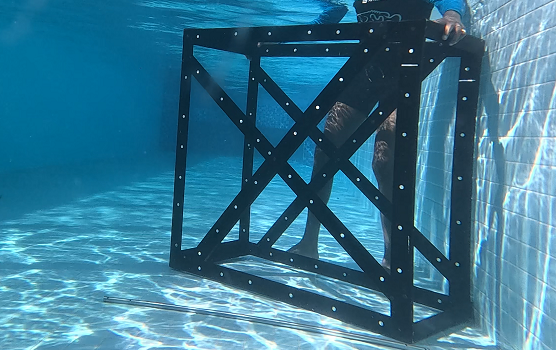
\includegraphics[keepaspectratio]{images/clipboard-1368029145.png}}
\item
  Atenção! Durante as operações de piscina, o operador do cubo e o
  supervisor da operação precisam tem muito cuidado durante o manuseio
  do cubo para que as mão do operador não cubram algum dos pontos do
  cubo. Conforme aconteceu abaixo, onde a mão direita do operador está
  encobrindo o ponto 240:

  \pandocbounded{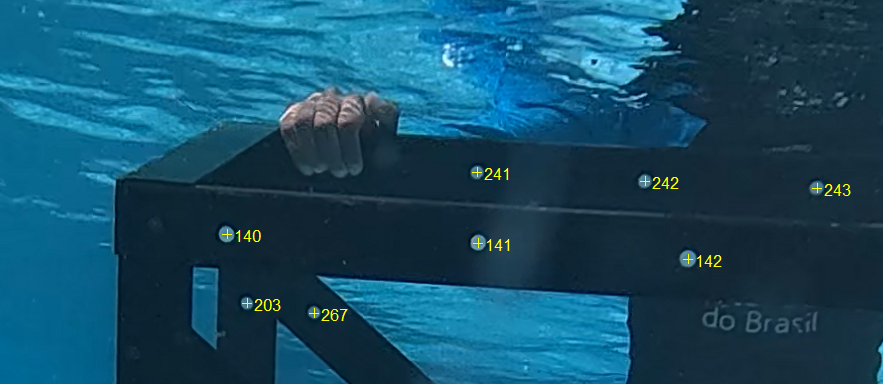
\includegraphics[keepaspectratio]{images/clipboard-1918781238.png}}
\end{enumerate}

\section{Mudando as cores}\label{mudando-as-cores}

Você pode mudar as cores dos pontos, já que a cor dos pontos não
residuais (pontos azuis) é de difícil distinção no fundo azul da
piscina. Isso irá ajudar a minimizar os erros. Se quiser mudar, vá em
\emph{Ajustement} \textgreater{} \emph{Point colors\ldots{}}

\pandocbounded{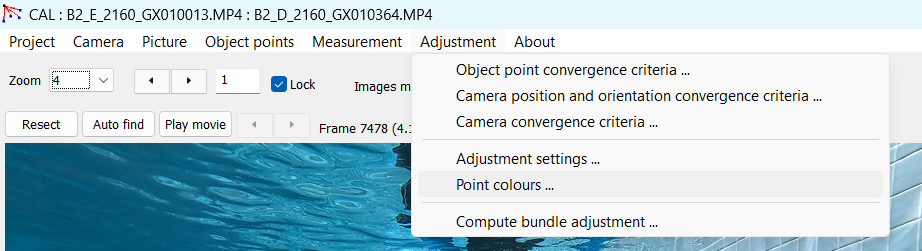
\includegraphics[keepaspectratio]{images/clipboard-3756644147.png}}

Uma pequena janela se abrirá mostrando as cores padrões:

\pandocbounded{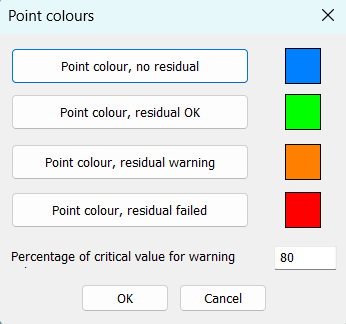
\includegraphics[keepaspectratio]{images/clipboard-3887801960.png}}

Clique em \emph{Point colour, no residual} e altere para a cor que
desejar (ex: amarelo):

\pandocbounded{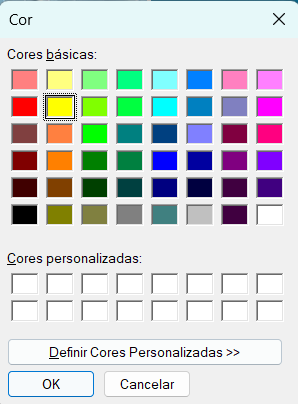
\includegraphics[keepaspectratio]{images/clipboard-2013230235.png}}

Antes:

\pandocbounded{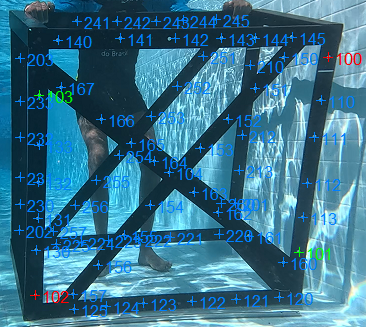
\includegraphics[keepaspectratio]{images/clipboard-168867011.png}}

Depois:

\pandocbounded{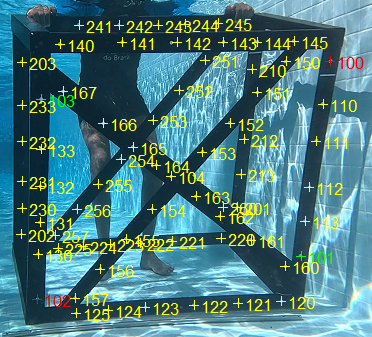
\includegraphics[keepaspectratio]{images/clipboard-4114342458.png}}

\section{Finalizando os trabalhos}\label{finalizando-os-trabalhos}

\begin{enumerate}
\def\labelenumi{\arabic{enumi}.}
\tightlist
\item
  Ao final do processo de medição (marcações de pontos), você deverá ter
  um total de 40 images (20 câmera esquerda e 20 câmera direita). Você
  poder ver isso na própria tela principal do programa, onde há um campo
  descrito como \emph{Images measured:}
\end{enumerate}

\begin{center}
\pandocbounded{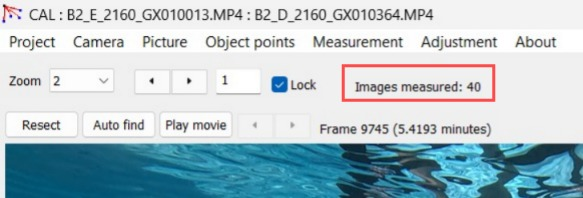
\includegraphics[keepaspectratio]{images/WhatsApp Image 2026-03-19 at 09.56.23.jpeg}}
\end{center}

\begin{enumerate}
\def\labelenumi{\arabic{enumi}.}
\setcounter{enumi}{1}
\item
  Estando tudo certo, iremos partir para o \textbf{ajuste do
  feixe}\footnote{Ajuste do Feixe: Tradução livre de \emph{Bundle
    Adjustement,} termo utilizado na área de fotogrametria e visão
    computacional que se refere a um processo de otimização matemática
    para melhorar a reconstrução 3D de uma cena a partir de multiplas
    imagens. Tecnicamente, é um problema de mínimos quadrados não
    lineares, onde minimiza-se o erro da reprojeção.} ou \emph{bundle
  adjustment.}
\item
  Mas antes é importante saber que você pode ajustar os parâmentros do
  ajuste (\emph{bundle adjustment}) no menu \emph{Adjustment \textbar{}
  Adjustment setting\ldots{}}

  \pandocbounded{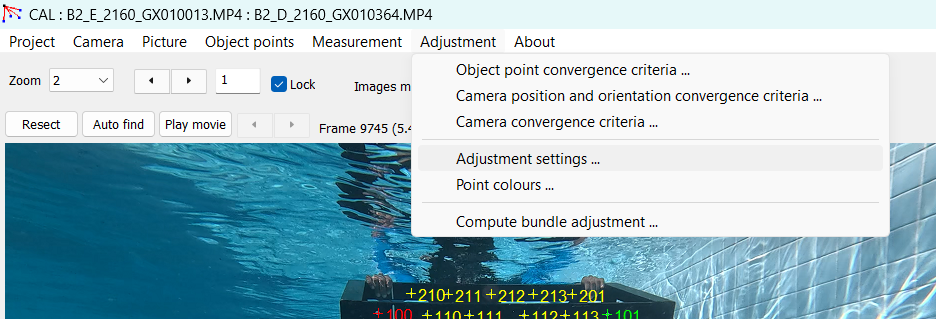
\includegraphics[keepaspectratio]{images/clipboard-554416799.png}}
\item
  Acho que o mais importante aqui é avisar ao programa que estamos
  utilizando um sistema estéreo (\emph{Stereo}-BRUV) e, portanto, exigir
  dele um restrição estéreo (\emph{stereo constraint})

  \begin{tcolorbox}[enhanced jigsaw, opacityback=0, toprule=.15mm, colframe=quarto-callout-tip-color-frame, arc=.35mm, breakable, rightrule=.15mm, left=2mm, leftrule=.75mm, colback=white, bottomrule=.15mm]
  \begin{minipage}[t]{5.5mm}
  \textcolor{quarto-callout-tip-color}{\faLightbulb}
  \end{minipage}%
  \begin{minipage}[t]{\textwidth - 5.5mm}

  Se você não sabe se o BRUV que está utilizando é estéreo, assista esse
  pequeno vídeo para noções basicas de fotogrametria:
  \url{https://www.youtube.com/watch?v=BZdzyzMjAjc}

  \end{minipage}%
  \end{tcolorbox}
\item
  Clicando em \emph{Adjustment \textbar{} Adjustment setting}, abrirá um
  a janela (\emph{Adjustment and photogrammetry settings)} contendo uma
  tabela com quatro colunas:

  \pandocbounded{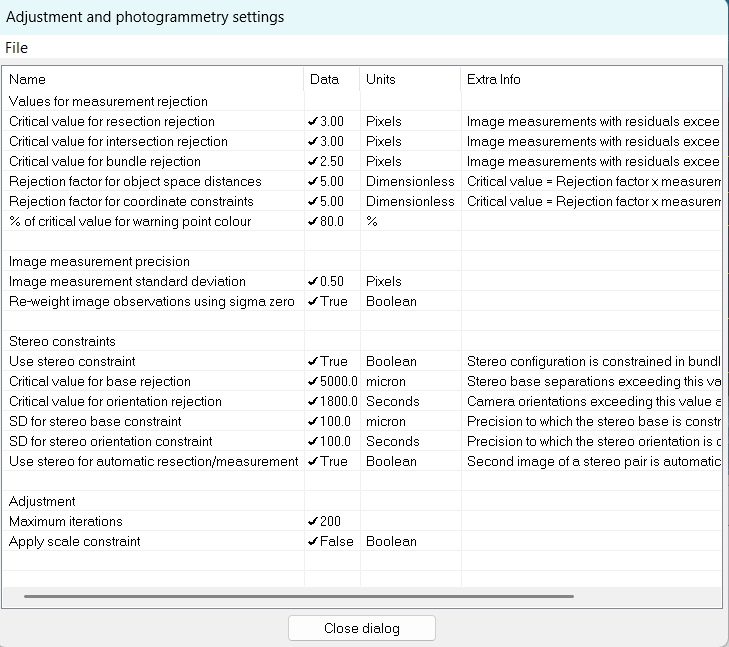
\includegraphics[keepaspectratio]{images/clipboard-1526197752.png}}
\item
  Perceba que essa tabela possui quatro seções:

  \pandocbounded{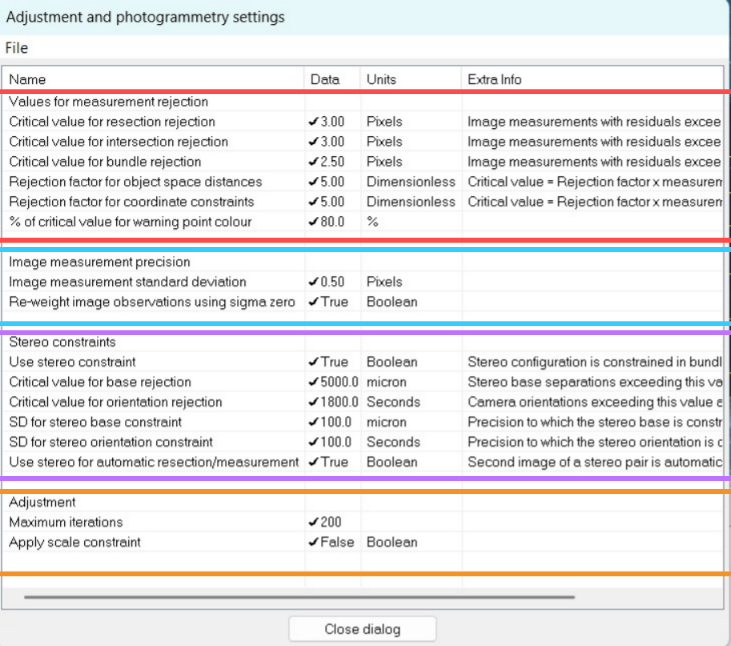
\includegraphics[keepaspectratio]{images/image.png}}
\item
  Na seção roxa ou 3° seção (\emph{Stereo constraints}), temos na
  primeira linha (\emph{Use stereo constraint)} como padrão
  (\emph{default}), \emph{False.}
\end{enumerate}

\begin{verbatim}
::: {.callout-warning appearance="simple"}
Perceba que isso que falo não está expresso nas duas ultimas fotos anteriores, pois já havia realizado a mudança quando realizei o recorte, mas mantive para me poupar trabalho.
:::
\end{verbatim}

\begin{enumerate}
\def\labelenumi{\arabic{enumi}.}
\setcounter{enumi}{7}
\item
  Selecione a célula da coluna \emph{Data} e mude para
  \textbf{\emph{True}} (escreva!).

  \pandocbounded{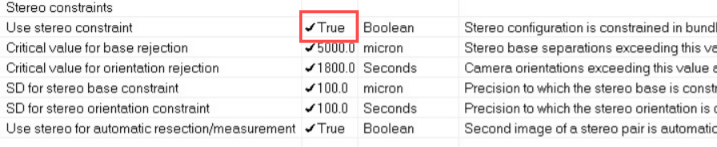
\includegraphics[keepaspectratio]{images/image (1).png}}
\item
  Isso impõe condições matemáticas ao \emph{bundle adjustment} que
  obrigam os pares de imagens (esquerda/direita) a manter a mesma
  orientação relativa ao longo de todo conjunto de imagens, forçando
  consistência na geometria relativa entre as duas câmeras (par
  estéreo).
\item
  Se esse for seu caso (Stereo-Bruvs), feito isso, seguimos para o
  ajuste de feixe.
\end{enumerate}

\subsection{Ajuste do Feixe}\label{ajuste-do-feixe}

\begin{enumerate}
\def\labelenumi{\arabic{enumi}.}
\item
  Após concluir todas as medições (marcações de pontos), calcule o
  ajuste do feixe usando \emph{Adjustment} \textbar{} \emph{Compute
  bundle adjustment\ldots{}}

  \pandocbounded{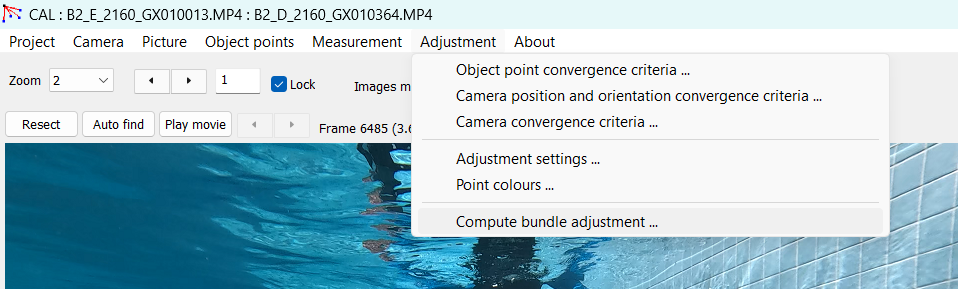
\includegraphics[keepaspectratio]{images/clipboard-959548070.png}}

  \begin{tcolorbox}[enhanced jigsaw, colbacktitle=quarto-callout-note-color!10!white, colframe=quarto-callout-note-color-frame, bottomtitle=1mm, title=\textcolor{quarto-callout-note-color}{\faInfo}\hspace{0.5em}{Note}, leftrule=.75mm, coltitle=black, bottomrule=.15mm, opacityback=0, toprule=.15mm, toptitle=1mm, opacitybacktitle=0.6, arc=.35mm, breakable, titlerule=0mm, rightrule=.15mm, colback=white, left=2mm]

  O QUE É ``FEIXE'' (\emph{BUNDLE})?

  Cada ponto 3D projeta um conjunto de linha (x, y, z) (ou um feixe/
  pacote de raios) em direção às diferentes câmeras.

  \end{tcolorbox}
\item
  Se você receber uma mensagem de aviso sobre medições de distância
  excluídas ou baixa precisão relativa, ignore-a por enquanto.

  \pandocbounded{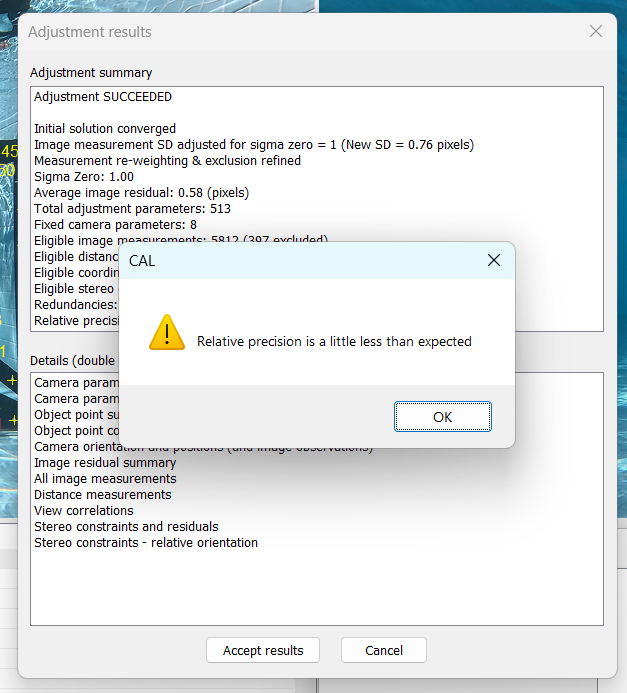
\includegraphics[keepaspectratio]{images/clipboard-2851610986.png}}
\item
  Se o ajuste falhar, consulte os motivos pelos quais um ajuste de feixe
  pode falhar no manual. Se ainda estiver com dificuldades para obter
  resultados que não convergem, tente uma solução apenas com a face
  frontal, descrita na seção \textbf{Falha de ajustes com um cubo de
  calibração SeaGIS}.

  \pandocbounded{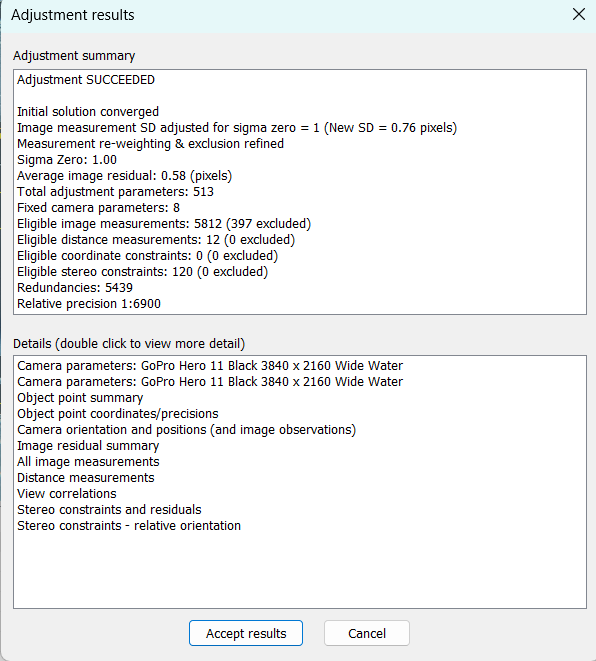
\includegraphics[keepaspectratio]{images/clipboard-2208317373.png}}
\item
  Uma vez analisado os resultados e apurado as mensagens \emph{warning,}
  clique em \emph{Acepted results}. (Por sua conta em risco).
\end{enumerate}

Salvamento Arquivo

\begin{enumerate}
\def\labelenumi{\arabic{enumi}.}
\item
  Feito isso, agora vamos salvar o arquivo.
\item
  Clique em \emph{Measurement} \textbar{} \emph{Write measurement
  file\ldots{}}

  \pandocbounded{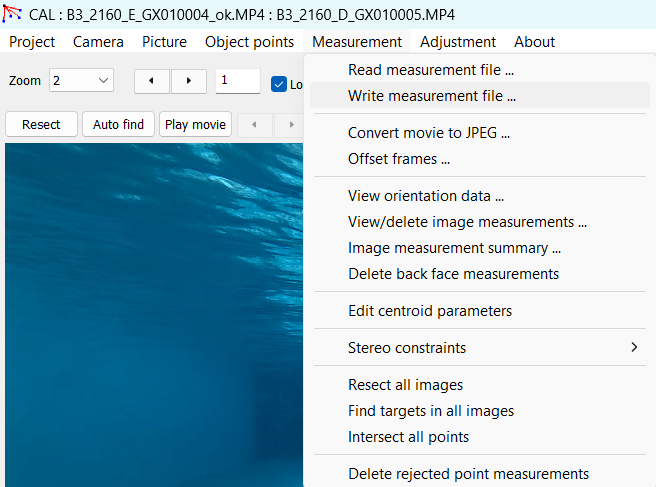
\includegraphics[keepaspectratio]{images/clipboard-768242398.png}}
\item
  Renomeie o arquivo conforme exemplo abaixo e salve no diretório de
  trabalho.

  \pandocbounded{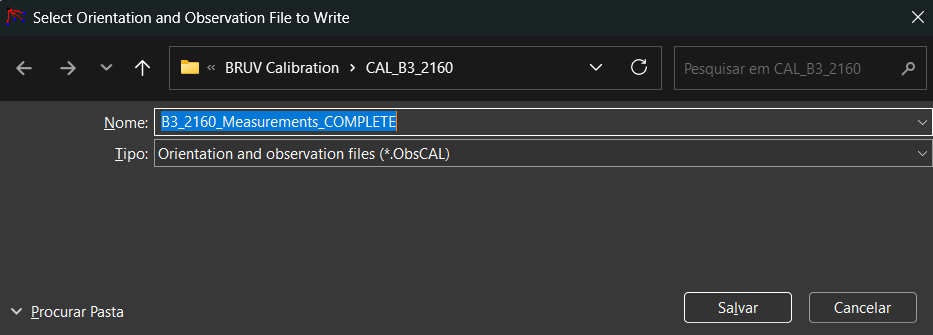
\includegraphics[keepaspectratio]{images/clipboard-3631012630.png}}
\item
  Parabéns, você concluío!
\end{enumerate}

\section{Detectando Erros}\label{detectando-erros}

É muito comum, por falta de conhecimento e prática ou até total
desconhecimento do que está sendo feito, erros de atenção. O mais comum
dele é ``saltar'' uma das sequências de transição do cubo de calibração
(Ver Item 21). A esse tipo de erro, eu chamo de ``erro de transição''.

\section{Erro de Transição}\label{erro-de-transiuxe7uxe3o}

O erro de transição pode ou não comprometer todo o processo de
calibração do sistema \emph{stereo-bruv}. Isso vai depender se ao final
do processo de ajuste de feixe teremos um ajuste bem sucedido ou não
(Item 2, Ajuste de Feixe). Vai depender do operador descidir proceguir
ou não com os trabalhos para verificar se vai ser valido ou não. A
depender da quantidade de sequência omitida não vale a pena continuar, e
será nescessário retornar a piscina e refazer todo o processo do começo.
Por isso preste atenção e não erre. Na seção seguinte, veremos o que
fazer quando deterctar um erro.

\section{Error Report}\label{error-report}

\begin{enumerate}
\def\labelenumi{\arabic{enumi}.}
\tightlist
\item
  Durante os trabalhos, quando você se deparar com um erro, pause seu
  trabalho e anote em sua carderneta pessoal as seguintes informações:
  ``\emph{Dia-Bruv-Processo-Referência-Frame-Erro}'', por exemplo:
\end{enumerate}

\pandocbounded{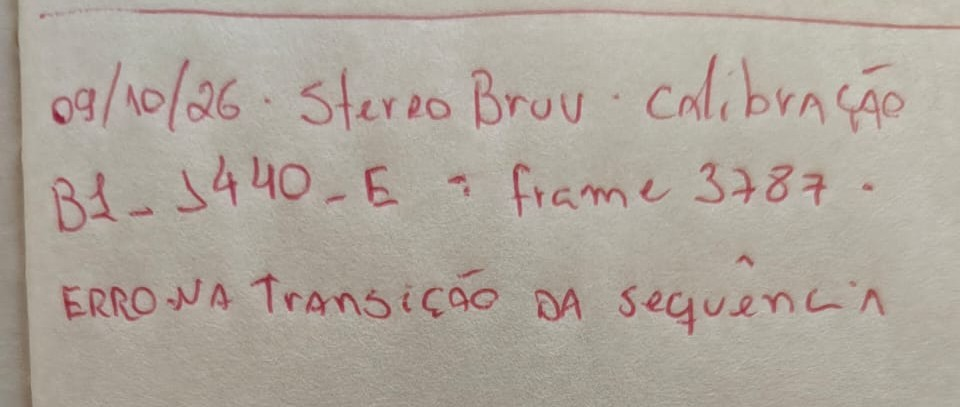
\includegraphics[keepaspectratio]{images/WhatsApp Image 2026-10-09 at 10.21.58.jpeg}}

\begin{enumerate}
\def\labelenumi{\arabic{enumi}.}
\setcounter{enumi}{1}
\tightlist
\item
  Depois faça salve uma imagem (.png) do slide de referência em uso
  adicionando o título de referência e o ``error'' na posição que seria
  seguida, conforme abaixo:
\end{enumerate}

\pandocbounded{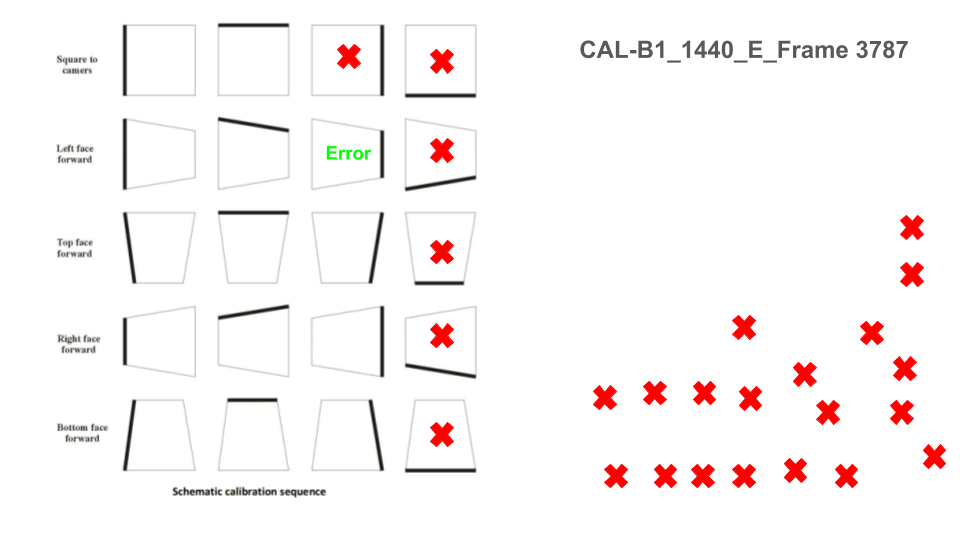
\includegraphics[keepaspectratio]{images/261009_B1_1449_E_3787.png}}

\begin{enumerate}
\def\labelenumi{\arabic{enumi}.}
\setcounter{enumi}{2}
\item
  Renomei a imagem com: \emph{data ao contrário (ano/mês/dia),
  referência do bruv, resolução do bruv, posição do bruv e frame.}
  Exemplo: \textbf{261009\_B1\_1440\_E\_3787}.
\item
  Transfira a imagem salva para o drive do projeto.
\item
  No nosso caso é: \textbf{Pesquisa SC \textgreater{}
  Calibragem-CALProgram-SeaGIS \textgreater Erros}
\item
  Agora realize o \emph{Error} \emph{Report.} Utilize o modelo
  \emph{report.qmd.}
\item
  Modelo html:

  \pandocbounded{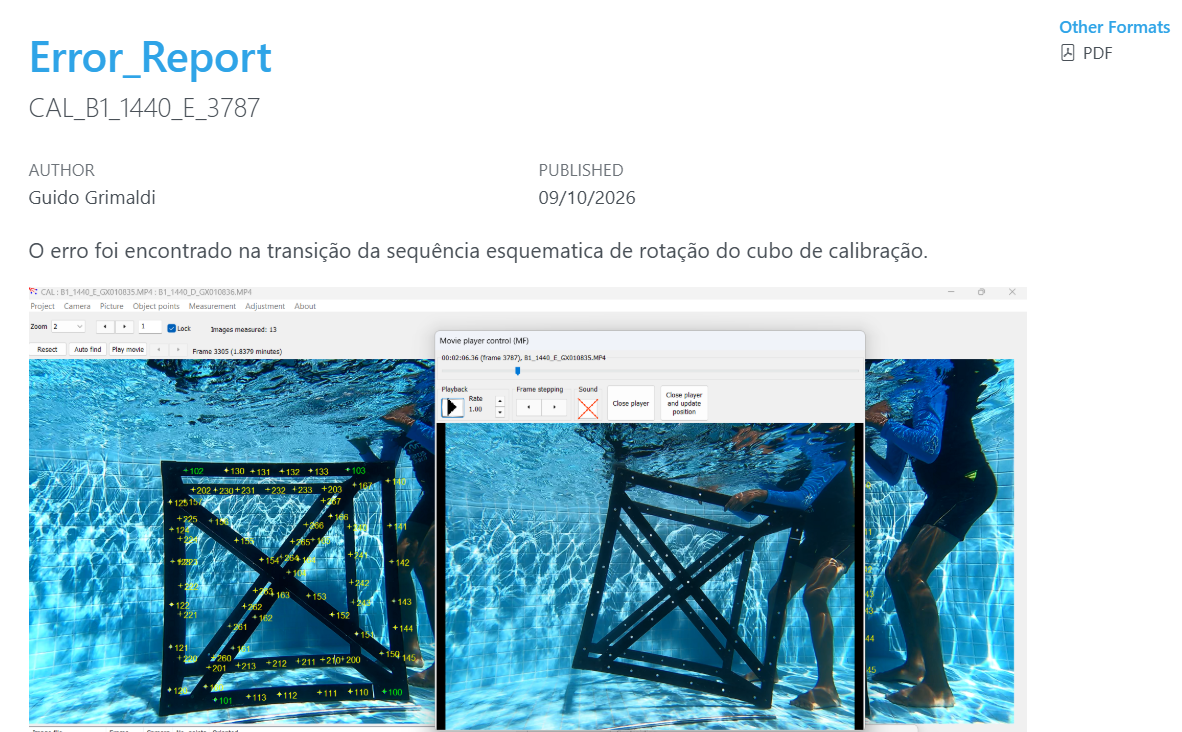
\includegraphics[keepaspectratio]{images/clipboard-3282701280.png}}
\item
  Modelo pdf:

  \pandocbounded{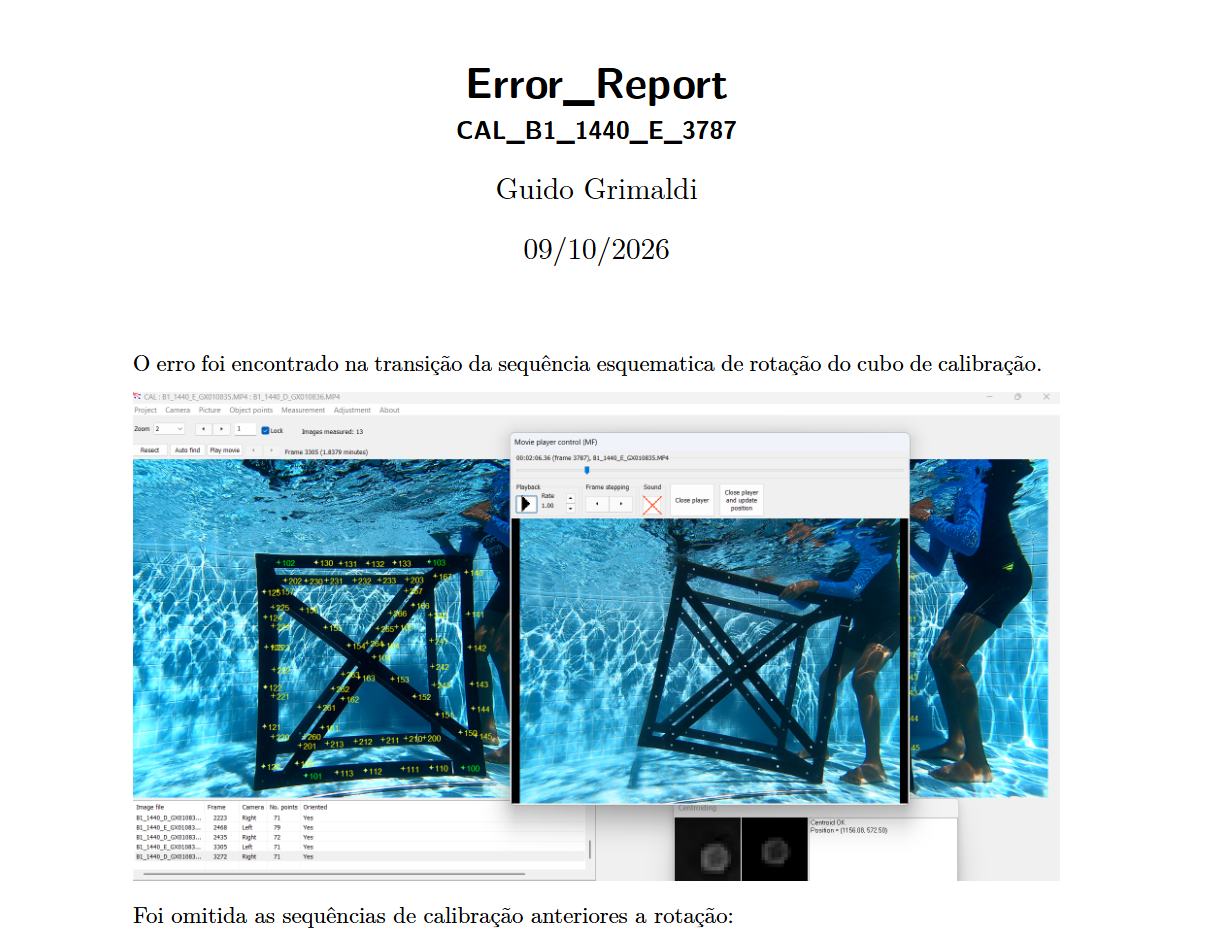
\includegraphics[keepaspectratio]{images/clipboard-2551310356.png}}
\item
  Ou construa o seu, o importante é conter uma \textbf{imagem da tela de
  trabalho} no momento da detecção do erro e outra \textbf{imagem do
  guia de acompanhamento} das transições esquemáticas.
\item
  Não esqueça de datar e assinar seu nome.
\item
  Envie o relatório ao seu coordenador.
\end{enumerate}

\section{Glossário}\label{glossuxe1rio}

Ajuste do Feixe: Tradução livre de \emph{Bundle Adjustement,} termo
utilizado na área de fotogrametria e visão computacional que se refere a
um processo de otimização matemática para melhorar a reconstrução 3D de
uma cena a partir de multiplas imagens. Tecnicamente, é um problema de
mínimos quadrados não lineares, onde minimiza-se o erro da reprojeção.




\end{document}
